% Portions Copyright (c) 2005 Nokia Corporation
\documentclass{manual}

% NOTE: this file controls which chapters/sections of the library
% manual are actually printed.  It is easy to customize your manual
% by commenting out sections that you're not interested in.

\title{PyS60 Library Reference}

\input{boilerplate}

\makeindex                      % tell \index to actually write the
                                % .idx file
\makemodindex                   % ... and the module index as well.

%begin{latexonly}
\ifx\pdftexversion\undefined
 \usepackage[dvips]{graphicx}
\else
 \usepackage[pdftex]{graphicx}
\fi
%end{latexonly}
\usepackage{graphicx}

\usepackage{longtable}

\graphicspath{{./}{figures/}}

\begin{document}

\maketitle

\ifhtml
\chapter*{Front Matter\label{front}}
\fi

\input{copyright}

\begin{abstract}

\noindent

The Python for S60 Platform (Python for S60) simplifies application development 
and provides a scripting solution for the Symbian C++ APIs. This document is for 
Python for S60 version \productversion that is based on Python 2.2.2.

\end{abstract}

\tableofcontents

                                % Chapter title:

% Copyright (c) 2005 Nokia Corporation
%
% Licensed under the Apache License, Version 2.0 (the "License");
% you may not use this file except in compliance with the License.
% You may obtain a copy of the License at
%
%     http://www.apache.org/licenses/LICENSE-2.0
%
% Unless required by applicable law or agreed to in writing, software
% distributed under the License is distributed on an "AS IS" BASIS,
% WITHOUT WARRANTIES OR CONDITIONS OF ANY KIND, either express or implied.
% See the License for the specific language governing permissions and
% limitations under the License.

\chapter{Introduction}
\label{intro}

% XXX add macro version here
The Python for S60 Platform (Python for S60) simplifies 
application development and provides a scripting solution for the Symbian 
C++ APIs. This document is for Python for S60 release 1.3.1 that is 
based on Python 2.2.2.

The documentation for Python for S60 includes three documents:

\begin{itemize}
\item Getting Started with Python for S60 Platform \cite{PyS60Start} contains information on how to install Python for S60 and how to write your first program.
\item This document contains API and other reference material.
\item Programming with Python for S60 Platform \cite{PyS60Prog} contains code examples and programming patterns for S60 devices that can be used as a basis for programs.
\end{itemize}
Python for S60 as installed on a S60 device consists of:

\begin{itemize}
\item Python execution environment, which is visible in the application menu of the device and has been written in Python on top of Python for S60 Platform (see S60 SDK documentation \cite{S60Doc})
\item Python interpreter DLL
\item Standard and proprietary Python library modules
\item S60 UI application framework adaptation component (a DLL) that connects the scripting domain components to the S60 UI
\item Python Installer program for installing Python files on the device, which consists of:
	\begin{itemize}
	\item Recognizer plug-in
	\item Symbian application written in Python
	\end{itemize}
\end{itemize}

The Python for S60 developer discussion board \cite{PyS60DiBo} on the 
Forum Nokia Web site is a useful resource for finding out information on 
specific topics concerning Python for S60. You are welcome to give 
feedback or ask questions about Python for S60 through this discussion 
board.

\section{Scope}
\label{subsec:scope}

This document includes the information required by developers to create 
applications that use Python for S60, and some advice on extending the 
platform.

\section{Audience}
\label{subsec:audience}

This guide is intended for developers looking to create programs that use the 
native features and resources of the S60 phones. The reader should be 
familiar with the Python programming language (\url{http://www.python.org/}) and 
the basics of using Python for S60 (see Getting Started with Python for 
S60 Platform \cite{PyS60Start}).

% XXX version macro to this declaration
\section{New in Release 1.3.1}
\label{subsec:new}

% XXX macro could include version-1 also
This section lists the updates in this document since release 1.2.

\begin{itemize}
\item New attribute \code{focus}, \ref{subsec:application}, Application Type.
\item Support for float values in \code{query} and \code{Form}, \ref{subsec:module}, Module Level Functions and \ref{subsec:form}, Form Type respectively.
\item Global note in \code{note}, \ref{subsec:module}, Module Level Functions.
\item Setting the device time, \ref{subsec:e32}, Module Level Functions.
\item New type \code{Ao_timer}, \ref{subsec:Aotimer}, Ao\_timer Type.
\item Section \ref{sec:inbox}, \code{inbox} Module has been added.
\item New functionality in \code{Sound}, \ref{subsec:sound}, Sound Objects.
\end{itemize}

\section{Naming Conventions}
\label{subsec:naming}

Most names of the type \code{ESomething} typically indicate a constant defined 
by the Symbian SDK. More information about these constants can be found in the 
Symbian SDK documentation.
                % Introduction

% Copyright (c) 2005 Nokia Corporation
%
% Licensed under the Apache License, Version 2.0 (the "License");
% you may not use this file except in compliance with the License.
% You may obtain a copy of the License at
%
%     http://www.apache.org/licenses/LICENSE-2.0
%
% Unless required by applicable law or agreed to in writing, software
% distributed under the License is distributed on an "AS IS" BASIS,
% WITHOUT WARRANTIES OR CONDITIONS OF ANY KIND, either express or implied.
% See the License for the specific language governing permissions and
% limitations under the License.

\chapter{API Summary}
\label{sec:summary}

All built-in object types of the Python language are supported in the
S60 environment. The rest of the programming interfaces are
implemented by various library modules as summarized in this chapter.

\section{Python Standard Library}
\label{subsec:python}

% XXX appendix reference
Python for S60 platform distribution does not include all of the 
Python's standard and optional library modules to save storage space in the 
phone. Nevertheless, many of the excluded modules also work in the S60 
Python environment without any modifications. Some modules are included in 
the SDK version but not installed in the phone. For a summary of supported 
library modules, see Chapter \ref{s60lib}.

When Python, available at \url{http://www.python.org/}, is installed on a PC, the 
library modules are by edefault located in \file{\textbackslash Python22\textbackslash Lib}
on Windows and in \file{/usr/lib/python2.2} on Linux. The Python library 
modules' APIs are documented in \cite{PyLibRef}.

Python for S60 extends some standard modules. These extensions are 
described in this document, see Chapter \ref{extensions}.

\section{Python for S60 Extensions}
\label{sec:sumext}

There are two kinds of native C++ extensions in the Python for S60 
Platform: built-in extensions and dynamically loadable extensions.

\subsection{Built-in extensions}
\label{sec:built}

There are two built-in extensions in the Python for S60 package:

\begin{itemize}
\item The \refmodule{e32} extension module is built into the Python interpreter on Symbian OS, and implements interfaces to special Symbian OS Platform services that are not accessible via Python standard library modules.
\item The \refmodule{appuifw} module for Python for S60 Platform offers UI application framework related Python interfaces.
\end{itemize}

\subsection{Dynamically loadable extensions}
\label{sec:dynamically}

These dynamically loadable extension modules provide proprietary APIs
to S60 Platform's services: \refmodule{graphics} (see Chapter
\ref{sec:graphics}, graphics Module), \refmodule{e32db} (see Chapter
\ref{sec:e32db}, e32db Module),
\refmodule{messaging} (see Chapter \ref{sec:messaging}, messaging Module), 
\refmodule{inbox} (see Chapter \ref{sec:inbox}, inbox Module), \refmodule{location} 
(see Chapter \ref{sec:location}, location Module), \refmodule{sysinfo} (see Chapter 
\ref{sec:sysinfo}, sysinfo Module), \refmodule{camera} (see Chapter 
\ref{sec:camera}, camera Module), \refmodule{audio} (see Chapter \ref{sec:audio}, 
audio Module), \refmodule{telephone} (see Chapter \ref{sec:telephone}, telephone 
Module), \refmodule{calendar} (see Chapter \ref{sec:calendar}, calendar Module), 
and \refmodule{contacts }(see Chapter \ref{sec:contacts}, contacts Module).

\section{Third-Party Extensions}
\label{subsec:third}

% XXX appendix references
It is also possible to write your own Python extensions. S60 related
extensions to Python/C API are described in Chapter
\ref{capiextensions}. For some further guidelines on writing
extensions in C/C++, see Chapter \ref{extending}. In
addition, for an example on porting a simple extension to S60, see
\cite{PyS60Prog}.
              % API summary

% Copyright (c) 2005 Nokia Corporation
%
% Licensed under the Apache License, Version 2.0 (the "License");
% you may not use this file except in compliance with the License.
% You may obtain a copy of the License at
%
%     http://www.apache.org/licenses/LICENSE-2.0
%
% Unless required by applicable law or agreed to in writing, software
% distributed under the License is distributed on an "AS IS" BASIS,
% WITHOUT WARRANTIES OR CONDITIONS OF ANY KIND, either express or implied.
% See the License for the specific language governing permissions and
% limitations under the License.

\chapter{Selected Issues on Python Programming for S60}
\label{sec:selected}

The following issues must be considered when using Python on S60.

\section{Concurrency Aspects}
\label{subsec:concurrency}
The thread that initializes the Python interpreter becomes the main Python 
thread. This is usually the main thread of a UI application. When an 
application written in Python launches, the Symbian platform infrastructure 
creates the main UI thread that starts the Python environment. If a Python 
program is started as a server with \code{e32.start_server}, then the 
Python main thread is not a UI thread.

It is possible to launch new threads via the services of \module{thread} 
module. Examples of such situations could be to overcome eventual problems 
with the fixed, relatively small stack size of the main UI application 
thread; or to perform some background processing while still keeping the UI 
responsive. These new threads are not allowed to directly manipulate the UI; 
in other words, they may not use the \module{appuifw} module.

Because of the limitations of the Python interpreter's final cleanup, Python 
applications on the Symbian OS should be designed in such a way that the 
main thread is the last thread alive.

A facility called active object is used extensively on the Symbian OS to 
implement co-operative, non-preemptive scheduling within operating system 
threads. This facility is also utilized with native APIs. A Python 
programmer is exposed to related concurrency issues particularly in UI 
programming. Preserving the responsiveness of the UI with the help of active 
objects needs to be considered when designing the application logic. At the 
same time it is necessary to take into account the resulting concurrent 
behavior within the application when active objects are used. While the main 
execution path of a UI script is blocked in wait for an active object to 
complete -- either explicitly as a result of using \code{e32.Ao_lock}, 
or indirectly within some other Python API implementation -- the UI-related 
callbacks may still get called.

The standard \code{thread.lock} cannot normally be used for 
synchronization in the UI application main thread, as it blocks the UI event 
handling that takes place in the same thread context. The Symbian active 
object based synchronization service called \code{e32.Ao_lock} has been 
implemented to overcome this problem. The main thread can wait in this lock, 
while the UI remains responsive.

Python for S60 tries to minimize the unwanted exposure of a Python 
programmer to the active objects of the Symbian OS. The programmer may 
choose to implement the eventual concurrent behavior of the application with 
normal threads. However, certain active object based facilities are offered 
as an option in the \module{e32} module.

\section{Current S60 Python Script Execution Environment}
\label{subsec:current}

The current options for installing Python scripts to a S60 device are: a 
stand-alone installation to the device's main application menu, and an 
installation to a folder hierarchy maintained by the Python execution 
environment. For more details on this topic, see Programming with Python for 
S60 Platform \cite{PyS60Prog}. In the first case the script application is 
launched via application menu, and it executes in its own process context. The 
latter case is suitable for development, testing, and trying out new scripts.

The Python execution environment delivered with Python for S60 package 
has itself been written in Python. It is a collection of scripts that offer 
an interactive Python console and a possibility to execute scripts located 
in the directory of the execution environment. Due to this kind of design 
the scripts are not fully isolated from each other. This means that any 
changes a script makes in the shared execution environment are visible to 
other scripts as well. This may be helpful during the development of a 
script suite, as long as care is taken to avoid unwanted interference 
between scripts.

For some special issues to consider when writing Python scripts to be run from 
the current Python execution environment, see Programming with Python for S60 Platform \cite{PyS60Prog}. These include the arrangements for standard output 
and the maintenance of the Options menu contents.

\section{Standard I/O Streams}
\label{subsec:standard}

The standard Python I/O streams in the \module{sys} module are by default 
connected to underlying C STDLIB's \code{stdio} streams that in turn are 
terminated by dummy file descriptors. Usually Python scripts set the I/O 
streams suitably by manipulating them at Python level via \module{sys} 
module interface. The \module{e32} extension module offers a Python 
interface for attaching to C STDLIB's output streams, but this service is 
only recommended for debugging purposes. The \code{e32._stdo} function 
takes as its argument the name of the file where C STDLIB's \code{stdout} 
and \code{stderr} are to be redirected. This makes it possible to capture 
the low-level error output when the Python interpreter has detected a fatal 
error and aborts.

\section{Usage of Unicode}
\label{subsec:usage}
No changes have been made to the standard library modules with regard to 
string argument and return value types. S60 extensions generally 
accept both plain strings and Unicode strings as arguments, but they return 
only Unicode strings. APIs that take string arguments for the purpose of 
showing them on the UI expect Unicode strings. Giving something else may 
result in garbled appearance of the text on the screen.

\section{Date and Time}
\label{subsec:datetime}
Unix time, seconds since January 1, 1970, 00:00:00 UTC (Coordinated 
Universal Time), is generally used as the time format in the Python for 
S60 APIs described in this document. The float type is used for 
storing time values.

\section{Sharing Native Resources between Threads}
\label{subsec:sharing}

\begin{notice}[warning]
Python for S60 objects that wrap native resources cannot be shared
between threads. Trying this can lead to a crash. This is because
native resources cannot be shared between native threads. Examples:

\begin{itemize}
\item Symbian OS STDLIB implementation has some limitations that are reflected at OS module support (see S60 SDK documentation \cite{S60Doc}). For example, STDLIB file descriptors cannot be shared between threads, and for that reason, Python file objects cannot either. 
\item Sockets as implemented in the S60 version of the \module{socket} module.
\end{itemize}
\end{notice}

\section{Scalable User Interface}
\label{sec:scalable}

\begin{notice}[note]
S60 2nd Edition FP3 and further releases.
\end{notice}

S60 2nd Edition FP3 enables a new feature called scalable user interface. 
For Python developers scalable user interface is currently visible in new APIs 
supporting the scalable UI, icon loading, and new screen resolutions. For more 
information on scalable user interface, see Section \ref{subsec:icon}, Icon Type 
of this document, as well as Programming with Python for S60 Platform 
\cite{PyS60Prog}. 

\section{Error Handling}
\label{subsec:error}

The APIs described in this document may raise any standard Python 
exceptions. In situations where a Symbian error code is returned, its 
symbolic name is given as the value parameter of a \code{SymbianError} 
exception.

In case where the functions have nothing special to return, they return 
\code{None} on success.

\section{Limitations and Areas of Development}
\label{subsec:limitations}

Some OS level concepts to which the standard \module{os} library module 
offers an interface do not exist as such in Symbian OS environment. An 
example of this is the concept of current working directory.

Reference cycle garbage collection is not in use. Because of this, special 
care needs to be taken to dismantle cyclic references when a Python program 
exits. This prevents error messages related to native resources that are 
left open. The problem could be removed by developing support for collection 
of cyclic garbage or by performing a special cleanup action on interpreter 
exit. The \module{gc} module has been ported to the Symbian OS, and 
it has been verified to work. However, the current distribution has been 
built without \module{gc} support.
             % Selected issues

\chapter{Operating System Services and Information \label{s60os}}

\input{libe32}
\input{libsysinfo}

\chapter{User Interface and Graphics \label{s60graph}}

% Copyright (c) 2005 Nokia Corporation
%
% Licensed under the Apache License, Version 2.0 (the "License");
% you may not use this file except in compliance with the License.
% You may obtain a copy of the License at
%
%     http://www.apache.org/licenses/LICENSE-2.0
%
% Unless required by applicable law or agreed to in writing, software
% distributed under the License is distributed on an "AS IS" BASIS,
% WITHOUT WARRANTIES OR CONDITIONS OF ANY KIND, either express or implied.
% See the License for the specific language governing permissions and
% limitations under the License.

\newlength{\screenwidth}
\setlength{\screenwidth}{0.3\textwidth}

\section{\module{appuifw} ---
	 Interface to the S60 GUI framework}

\declaremodule{standard}{appuifw}
\platform{S60}
\modulesynopsis{Interface to the S60 GUI framework}

The \module{appuifw} module offers an interface to S60 UI application
framework. \figurename~\ref{fig:ui-overview} provides an overview of
the Python for S60 environment for UI application programming.

\note{The services of this interface may only be used in the context of 
the main thread, that is, the initial thread of a UI application script.}

\begin{figure}
\centering
\includegraphics[width=\textwidth]{ui-overview}
\caption{Python for S60 UI environment overview}
\label{fig:ui-overview}
\end{figure}

\subsection{Basics of appuifw Module}
\label{subsec:basics}
Figure \ref{fig:normal-uilayout} shows the layout of a S60 application 
UI in the normal screen mode and a summary of how it relates to the services 
available at the \module{appuifw} API. For alternative layouts, see 
Figure \ref{fig:alternate-uilayouts}.

\begin{figure}
\centering
%\includegraphics[width=0.7\textwidth]{screen-parts}
\includegraphics{screen-parts}
\caption{The different parts of the screen when using the 'normal' layout}
\label{fig:normal-uilayout}
\end{figure}

\begin{figure}
\centering
\includegraphics[width=\screenwidth]{layout-normal}
\includegraphics[width=\screenwidth]{layout-large}
\includegraphics[width=\screenwidth]{layout-full}
\caption{UI layouts. left: 'normal', middle: 'large', right: 'full'}
\label{fig:alternate-uilayouts}
\end{figure}

The main application window may be set up to be occupied by a UI control.

A multi-view application can show the different views as tabs in the 
navigation pane and react as the users navigate between tabs. 

Dialogs always take precedence over the usual UI controls and appear on top 
of them.

UI controls are implemented as Python types. These types are available:

\begin{itemize}
\item \class{Text}
\item \class{Listbox}
\item \class{Canvas}
\end{itemize}
UI controls appear on the screen as soon as an instance of the corresponding 
Python type is created and set to the body field (\var{app.body}) of the 
current application UI.

\class{Form} is a versatile dialog implemented as a type.

The \class{Content_handler} type facilitates interfacing to other UI
applications and common high-level UI components. It is based on the
notion that designated handlers can reduce UI application interaction
to operations on MIME-type content.

The following dialogs are implemented as functions:

\begin{itemize}
\item \function{note}
\item \function{query}
\item \function{multi_query}
\item \function{selection_list}
\item \function{multi_selection_list}
\item \function{popup_menu}
\end{itemize}
A dialog becomes visible as soon as the corresponding Python function has 
been called. The function returns with the eventual user input or 
information on the cancellation of the dialog. \class{Form} is an 
exception; it is shown when its \method{execute} method is called.

\subsection{Softkeys}
\label{subsec:softkeys}
The softkeys are managed by the underlying S60 Platform. When no
dialog is visible, the right softkey is bound to application exit and
the left one represents an Options menu. Python for S60 offers
an interface for manipulating the menu and for binding the Exit key to
a Python-callable object (see Section \ref{subsec:application}). 

The native code that implements a dialog also manages the softkeys of the 
dialog, typically OK and Cancel. When the user input needs to be validated 
before accepting it and dismissing the dialog, it is best to use 
\class{Form}.

\subsection{Module Level Functions}
\label{subsec:module}
The following free functions - functions that do not belong to any class 
- are defined in the \module{appuifw} module:

\begin{funcdesc}{available_fonts}{}
Returns a list (Unicode) of all fonts available in the device.
\end{funcdesc}

\begin{funcdesc}{query}{label, type\optional{, initial_value}}
Performs a query with a single-field dialog. The prompt is set to 
\var{label}, and the type of the dialog is defined by \var{type}. The 
value of \var{type} can be any of the following strings:

\begin{itemize}
\item \code{'text'}
\item \code{'code'}
\item \code{'number'}
\item \code{'date'}
\item \code{'time'}
\item \code{'query'}
\item \code{'float'}
\end{itemize}

The type of the optional \var{initial_value} parameter and the 
returned input depend on the value of \var{type}:

\begin{itemize}
\item For text fields, (\code{'text'}, \code{'code'}) it is Unicode
\item For number fields, it is numeric
\item For date fields, it is seconds since epoch rounded down to the nearest local midnight
\end{itemize}

A simple confirmation query and time query take no initial value and return 
\code{True/None} and seconds since local midnight, correspondingly. All 
queries return \code{None} if the users cancel the dialog. 

For \code{'float'} query the \var{initial_value} setting has no 
effect.
\end{funcdesc}


\begin{funcdesc}{multi_query}{label_1, label_2}
A two-field text (Unicode) input dialog. Returns the inputted values
as a 2-tuple. Returns \code{None} if the users cancel the dialog.
\end{funcdesc}

\begin{funcdesc}{note}{text\optional{, type\optional{, global}}}
Displays a note dialog of the chosen type with \var{text} 
(Unicode). The default value for \var{type} is \code{'info'}, which is 
automatically used if \var{type} is not set. \var{type} can be one of 
the following strings: \code{'error'}, \code{'info'}, or 
\code{'conf'}. 

If \var{global} (integer) is any other value than zero a global note is 
displayed. A global note is displayed even if the Python application calling 
this function is in background. The same set of \var{type}s is supported as in 
standard note.
\end{funcdesc}

\begin{funcdesc}{popup_menu}{list\optional{, label}}
A pop-up menu style dialog. \var{list} representing the menu 
contents can be a list of Unicode strings or a list of Unicode string pairs 
(tuples). The resulting dialog list is then a single-style or a double-style 
list. A single-style list is shown in full; whereas a double-style list 
shows the items one at a time. Returns \code{None} if the user cancels the 
operation.
\end{funcdesc}

\begin{funcdesc}{selection_list}{choices\optional{, search_field=0}}
Executes a dialog that allows the users to select a list item and
returns the \var{index} of the chosen item, or \code{None} if the
selection is cancelled by the users. \var{choices} is a list of
Unicode strings.
\var{search_field} is \code{0} (disabled) by default and is optional. Setting it to \code{1} enables a search field (find pane) that facilitates searching for items in long lists. If enabled, the search field appears after you press a letter key.
\end{funcdesc}

\begin{funcdesc}{multi_selection_list}{choices\optional{, style='checkbox', search_field=0}}
  Executes a dialog that allows the users to select multiple list
  items.  Returns a tuple of indexes (a pair of Unicode strings) of
  the chosen items, or \code{None} if the selection is cancelled by
  the users. \var{choices} is a list of Unicode strings.  \var{style}
  is an optional string; the default value being \code{'checkbox'}.
  If \code{'checkbox'} is given, the list will be a checkbox list,
  where empty checkboxes indicate what items can be marked. The other
  possible value that can be set for \var{style} is
  \code{'checkmark'}. If \code{'checkmark'} is given, the list will be
  a markable list, which lists items but does not indicate
  specifically that items can be selected. To select items on a
  markable list, use the Navigation key to browse the list and the
  Edit key to select an item. For example views on checkbox and
  markable lists, see
  \figurename~\ref{fig:checkbox-and-markable-list}.
  \var{search_field} is \code{0} (disabled) by default and is
  optional. Setting it to \code{1} enables a search field (find pane)
  that facilitates searching for items in long lists. If enabled, the
  search field is always visible with checkbox lists; with markable
  lists it appears by pressing a letter key.

Example:
\begin{verbatim}
tuple = appuifw.multi_selection_list(L, style='checkmark', search_field=1)
\end{verbatim}
\end{funcdesc}

\begin{figure}[htbp]
\centering
\includegraphics[width=\screenwidth]{checkbox-list}
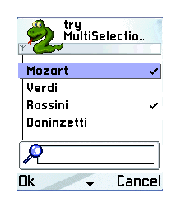
\includegraphics[width=\screenwidth]{markable-list}
\caption{Examples of a checkbox list (left) and a markable list (right)}
\label{fig:checkbox-and-markable-list}
\end{figure}

\subsection{Application Type}
\label{subsec:application}
A single implicit instance of this type always exists when \module{appuifw} 
module is present and can be referred to with the name \code{app}. New 
instances cannot be created by a Python program.

\begin{classdesc*}{Application}
Instances of \class{Application} type have the following attributes:

\begin{memberdesc}[Application]{body}
The UI control that is visible in the application's main window. Currently 
either \class{Text}, a \class{Listbox} object, \class{Canvas}, or 
\code{None}.
\end{memberdesc}

\begin{memberdesc}[Application]{exit_key_handler}
A callable object that is called when the user presses the Exit softkey. 
Setting \member{exit_key_handler} to \code{None} sets it back to the 
default value.
\end{memberdesc}

\begin{memberdesc}[Application]{menu}
This is a list of the following kinds of items:
\begin{itemize}
\item \code{(title, callback)} which creates a regular menu item
\item \code{(title, ((title, callback)\optional{...}))} which creates a submenu
\end{itemize}

\var{title} (Unicode) is the name of the item and \var{callback} the associated callable object. 
The maximum allowed number of items in a menu, or items in a submenu,
or submenus in a menu is 30.

Example:
\begin{verbatim}
appuifw.app.menu = [(u"Item 1", item1),
                    (u"Submenu 1", 
                        ((u"Subitem 1", subitem1),
                         (u"Subitem 2", subitem2)))]
\end{verbatim}
\end{memberdesc}

\begin{memberdesc}[Application]{screen}
The screen area used by an application. See \figurename~\ref{fig:alternate-uilayouts} for
example screens. The appearance of the application on the screen can
be affected by setting one of the following values: \code{'normal'},
\code{'large'}, and \code{'full'}.

Examples:
\begin{verbatim}
appuifw.app.screen='normal' # (a normal screen with title pane and softkeys)
appuifw.app.screen='large'  # (only softkeys visible)
appuifw.app.screen='full'   # (a full screen)
\end{verbatim}
\end{memberdesc}

\begin{memberdesc}[Application]{title}
The title the application that is visible in the application's title
pane. Must be Unicode.
\end{memberdesc}

\begin{memberdesc}[Application]{focus}
A callable object that is called with integer as parameter (0 = focus lost, 
1 = focus regained) when the application receives focus or it is switched to 
background. Focus is received e.g. when the application is switched from 
background to foreground or when the focus is regained from screensaver. 
Similarly when the screensaver is displayed, focus is lost.

Examples:
\begin{verbatim}
>>> import appuifw
>>> def cb(fg):
...   if(fg):
...     print "foreground"
...   else:
...     print "background"
...
>>> appuifw.app.focus=cb
>>> # switch to background, following text is printed from callback:
>>> background
>>> # switch to foreground, following text is printed from callback:
>>> foreground
\end{verbatim}

\begin{notice}
An improper callback can cause adverse effects. If you, for example,
define a callback which takes no parameters you will receive
never-ending \exception{TypeError} exceptions on the Nokia 6600.
\end{notice}

\end{memberdesc}

Instances of \class{Application} type have the following methods:

\begin{methoddesc}[Application]{activate_tab}{index}
Activates the tab \var{index} counting from zero.
\end{methoddesc}

\begin{methoddesc}[Application]{full_name}{}
Returns the full name, in Unicode, of the native application in whose 
context the current Python interpreter session runs.
\end{methoddesc}

\begin{methoddesc}[Application]{set_exit}{}
Requests a graceful exit from the application as soon as the current script 
execution returns.
\end{methoddesc}

\begin{methoddesc}[Application]{set_tabs}{tab_texts\optional{,callback=None}}
Sets tabs with given names on them in the navigation bar; 
\var{tab_texts} is a list of Unicode strings. When the users 
navigate between tabs, \var{callback} gets called with the index 
of the active tab as an argument. Tabs can be disabled by giving an empty or 
one-item \var{tab_texts} list.
\end{methoddesc}

\end{classdesc*}

\subsection{Form Type}
\label{subsec:form}
\class{Form} implements a dynamically configurable, editable multi-field 
dialog. \class{Form} caters for advanced dialog use cases with requirements 
such as free selectability of the combination of fields, possibility of 
validating the user input, and automatically producing the contents of some 
dialog fields before allowing the closing of the dialog. 

\begin{classdesc}{Form}{fields\optional{, flags=0}}
Creates a \class{Form} instance.
\var{fields} is a list of \emph{field descriptors}: \code{(label, type\optional{, value})} where

\var{label} is a Unicode string

\var{type} is one of the following strings: 
\code{'text'}, \code{'number'}, \code{'date'}, \code{'time'}, \code{'combo'}
or \code{'float'}

\var{value}, depending on \var{type}: Unicode string, numeric, float (seconds 
since Unix epoch rounded down to the nearest local midnight), float (seconds 
since local midnight), \code{([choice_label ...], index)} of float. For 
\code{'float'} \var{type} the initial value setting might not be shown in the 
UI.
\end{classdesc}

\class{Form} can also be configured and populated after construction. The 
configuration flags are visible as an attribute. \class{Form} implements 
the list protocol that can be used for setting the form fields, as well as 
obtaining their values after the dialog has been executed.

Instances of \class{Form} type have the following attributes:

\begin{memberdesc}[Form]{flags}
This attribute holds the values of the various configuration flags. 
Currently supported flags are:

\begin{datadesc}{FFormEditModeOnly}
When this flag is set, the form remains in edit mode while \method{execute} 
runs.
\end{datadesc}

\begin{datadesc}{FFormViewModeOnly}
When this flag is set, the form cannot be edited at all.
\end{datadesc}

\begin{datadesc}{FFormAutoLabelEdit}
This flag enables support for allowing the end-users to edit the labels of 
the form fields.
\end{datadesc}

\begin{datadesc}{FFormAutoFormEdit}
This flag enables automatic support for allowing the end-users to add and 
delete the form fields. Note that this is an experimental feature and is not 
guaranteed to work with all SDK versions.
\end{datadesc}

\begin{datadesc}{FFormDoubleSpaced}
When this flag is set, double-spaced layout is applied when the form is 
executed: one field takes two lines, as the label and the value field are on 
different lines.
\end{datadesc}
\end{memberdesc}

\begin{memberdesc}[Form]{menu}
A list of \code{(title, callback)} pairs, where 
each pair describes an item in the form's menu bar that is active while the 
dialog is being executed. \var{title} (Unicode) is the name of 
the item and \var{callback} the associated callable object.
\end{memberdesc}

\begin{memberdesc}[Form]{save_hook}
This attribute can be set to a callable object that receives one argument 
and returns a Boolean value. It gets called every time the users want to 
save the contents of an executing \class{Form} dialog. A candidate list for 
new form content - a list representing the currently visible state of the 
UI - is given as an argument. The list can be modified by 
\member{save_hook}. If \member{save_hook} returns \code{True}, the 
candidate list is set as the new contents of the form. Otherwise, the form 
UI is reset to reflect the field list contained in \class{Form} object.
\end{memberdesc}

Instances of \class{Form} type have the following methods:

\begin{methoddesc}[Form]{execute}{}
Executes the dialog by making it visible on the UI.
\end{methoddesc}

\begin{methoddesc}[Form]{insert}{index, field_descriptor}
Inserts the field descriptor into the \class{Form} before the given \var{index}.
\end{methoddesc}

\begin{methoddesc}[Form]{pop}{}
Removes the last field descriptor from the \class{Form} and returns it.
\end{methoddesc}

\begin{methoddesc}[Form]{length}{}the number of field descriptors in the form.
\end{methoddesc}

The subscript notation \code{f[i]} can be used to access or modify the
i-th element of the form \code{f}. Same limitations as discussed above
in the context of the flag \constant{FFormAutoFormEdit} apply to
modifying a form while it is executing. The ability to change the
schema of a form while it is executing is an experimental feature.

\subsection{Text Type}
\label{subsec:mylabel5}
\class{Text} is a text editor UI control. For examples on the options 
available with \class{Text}, see Figure \ref{fig:text-styles}.

\begin{figure}[htbp]
\centering
\includegraphics[width=\screenwidth]{text-styles-1}
\includegraphics[width=\screenwidth]{text-styles-2}
\caption{Examples of the options available for Text type}
\label{fig:text-styles}
\end{figure}

Instances of \class{Text} type have the following attributes:

\begin{memberdesc}[Text]{color}
The color of the text. \code{color} supports the same color representation 
models as the \module{graphics} module. For the supported color 
representation models, see Section \ref{sec:graphics}.
\end{memberdesc}

\begin{memberdesc}[Text]{focus}
A Boolean attribute that indicates the focus state of the control. Editor 
control also takes the ownership of the navigation bar, and this feature is 
needed to enable the usage of this control in applications that use the 
navigation bar - for example, navigation tabs.
\end{memberdesc}

\begin{memberdesc}[Text]{font} 
The font of the text. There are two possible ways to set this attribute:

\begin{itemize}

\item Using a supported Unicode font, for example \code{u"Latin12"}. Trying to set a font which is not supported by the device has no effect. A list of supported fonts can be retrieved by using \function{appuifw.available_fonts}.

Example, setting font:
\begin{verbatim}
t = appuifw.Text()
t.font = u"albi17b" # sets font to Albi 17 bold
t.font = u"LatinPlain12" # sets font to Latin Plain 12
\end{verbatim}
\item Using one of the default device fonts that are associated with the following labels (plain strings):
\code{'annotation', 'title', 'legend', 'symbol', 'dense', 'normal'}
Example, setting font: 
\begin{verbatim}
t.font = "title" # sets font to the one used in titles
\end{verbatim}

Example, checking the currently set font: 
\begin{verbatim}
unicodeFont = t.font
\end{verbatim}
\end{itemize}

The attribute value retrieved is always a Unicode string. If the font has 
been set with a label, for example, \code{'title'}, the attribute will 
retrieve the font associated with that label. 
\end{memberdesc}

\begin{memberdesc}[Text]{highlight_color}
The highlight color of the text. \code{highlight_color} supports the 
same color representation models as the \module{graphics} module. For the 
supported color representation models, see Section \ref{sec:graphics}.
\end{memberdesc}

\begin{memberdesc}[Text]{style}
The style of the text. The flags for this attribute are defined in the 
\module{appuifw} module. These flags can be combined by using the binary 
operator \code{|}. The flags can be divided into two types: text style 
and text highlight. Text style flags can be freely combined with each other. 
However, one or more text style flags can be combined with only one text 
highlight flag. The flags are:

Text style:

\begin{datadesc}{STYLE_BOLD} 
Enables bold text.
\end{datadesc}

\begin{datadesc}{STYLE_UNDERLINE}
Enables underlined text.
\end{datadesc}

\begin{datadesc}{STYLE_ITALIC} 
Enables italic text.
\end{datadesc}

\begin{datadesc}{STYLE_STRIKETHROUGH } 
Enables strikethrough.
\end{datadesc}

Text highlight:

\begin{datadesc}{HIGHLIGHT_STANDARD}
Enables standard highlight.
\end{datadesc}

\begin{datadesc}{HIGHLIGHT_ROUNDED}
Enables rounded highlight.
\end{datadesc}

\begin{datadesc}{HIGHLIGHT_SHADOW}
Enables shadow highlight.
\end{datadesc}

Only one highlight is allowed to be used at once. Therefore, it is possible 
to combine only one highlight with one or more text styles.

Examples:
\begin{verbatim}
t = appuifw.Text()

# These and other similar values and combinations are valid:
t.style = appuifw.STYLE_BOLD
t.style = appuifw.STYLE_UNDERLINE
t.style = appuifw.STYLE_ITALIC
t.style = appuifw.STYLE_STRIKETHROUGH
t.style = (appuifw.STYLE_BOLD|
	   appuifw.STYLE_ITALIC|
	   appuifw.STYLE_UNDERLINE)

# These values are valid:
t.style = appuifw.HIGHLIGHT_STANDARD
t.style = appuifw.HIGHLIGHT_ROUNDED
t.style = appuifw.HIGHLIGHT_SHADOW

# This combination is NOT valid:
# Invalid code, do not try!
t.style = (appuifw.HIGHLIGHT_SHADOW|appuifw.HIGHLIGHT_ROUNDED)
\end{verbatim}
\end{memberdesc}

Instances of \class{Text} type have the following methods:

\begin{methoddesc}[Text]{add}{text}
Inserts the Unicode string \var{text} to the current cursor position.
\end{methoddesc}

\begin{methoddesc}[Text]{bind}{event_code, callback}
Binds the callable Python object \var{callback} to event
\var{event_code}. The key codes are defined in 
the \module{key_codes} library module. The call 
\code{bind(event_code, None)} clears an 
existing binding. In the current implementation the event is always
passed also to the underlying native UI control.
\end{methoddesc}

\begin{methoddesc}[Text]{clear}{}
Clears the editor.
\end{methoddesc}

\begin{methoddesc}[Text]{delete}{\optional{pos=0, length=len()}}
Deletes \var{length} characters of the text held by the editor control, 
starting from the position \var{pos}.
\end{methoddesc}

\begin{methoddesc}[Text]{get_pos}{}
Returns the current cursor position.
\end{methoddesc}

\begin{methoddesc}[Text]{len}{}
Returns the length of the text string held by the editor control.
\end{methoddesc}

\begin{methoddesc}[Text]{get}{\optional{pos=0, length=len()}}
Retrieves \code{length} characters of the text held by the editor control, 
starting from the position \var{pos}.
\end{methoddesc}

\begin{methoddesc}[Text]{set}{text}
Sets the text content of the editor control to Unicode string 
\var{text}.
\end{methoddesc}

\begin{methoddesc}[Text]{set_pos}{cursor_pos}
Sets the cursor to \var{cursor_pos}.
\end{methoddesc}

\subsection{Listbox Type}
\label{subsec:listbox}

\begin{figure}[htbp]
\centering
\includegraphics[width=\screenwidth]{listbox-with-icons}
\caption{Listbox with icons}
\label{fig:listbox-with-icons}
\end{figure}

An instance of this UI control type is visible as a listbox, also known as a 
list in Symbian, that can be configured to be a single-line item or a 
double-item listbox. Figure \ref{fig:listbox-with-icons} shows a single-line 
item Listbox with icons. For more information on the MBM and MIF formats, 
see Section \ref{subsec:icon}.

\begin{classdesc}{Listbox}{list, callback}
Creates a \class{Listbox} instance. A callable object 
\var{callback} gets called when a listbox selection has been 
made. \code{list} defines the content of the listbox and can be one of the 
following:

\begin{itemize}
\item A normal (single-line item) listbox: a list of Unicode strings, for example \code{[unicode_string item1, unicode_string item2]}
\item A double-item listbox: a two-element tuple of Unicode strings , for example \code{[(unicode_string item1, unicode_string item1description), (unicode_string item2, unicode_string item2description)]}
\item A normal (single-line item) listbox with graphics: a two-element tuple consisting of a Unicode string and an \class{Icon} object, for example \code{[(unicode_string item1, icon1), (unicode_string item2, icon2)]}.
\item A double-item listbox with graphics: a three-element tuple consisting of two Unicode strings and one \class{Icon} object, for example \code{[(unicode_string item1, unicode_string item1description, icon1), (unicode_string item2, unicode_string item2description, icon2)]}
\end{itemize}

Example: To produce a normal (single-line item) listbox with graphics:
\begin{verbatim}
icon1 = appuifw.Icon(u"z:\\system\\data\\avkon.mbm", 28, 29)
icon2 = appuifw.Icon(u"z:\\system\\data\\avkon.mbm", 40, 41)
entries = [(u"Signal", icon1),
           (u"Battery", icon2)]
lb = appuifw.Listbox(entries, lbox_observe)
\end{verbatim}
\end{classdesc}

Instances of \class{Listbox} type have the following methods:

\begin{methoddesc}[Listbox]{bind}{event_code, callback}
Binds the callable Python object \var{callback} to event 
\var{event_code}. The key codes are defined in 
the \module{key_codes} library module. The call
\code{bind(event_code, None)} clears an 
existing binding. In the current implementation the event is always passed 
also to the underlying native UI control.
\end{methoddesc}

\begin{methoddesc}[Listbox]{current}{}
Returns the currently selected item's index in the \class{Listbox}.
\end{methoddesc}

\begin{methoddesc}[Listbox]{set_list}{list\optional{, current}}
Sets the \class{Listbox} content to a list of Unicode strings or a
list of tuples of Unicode strings. The accepted structures of \var{list} are the
same as in the \class{Listbox} constructor. The optional argument \var{current} is the index of the focused list item.
\end{methoddesc}

\subsection{Icon Type}
\label{subsec:icon}
An instance of \class{Icon} type encapsulates an icon to be used together 
with a \class{Listbox} instance. Note that currently \class{Icon} can only 
be used with \class{Listbox} (see Section \ref{subsec:listbox}).

MBM is the native Symbian OS format used for pictures. It is a
compressed file format where the files can contain several bitmaps and
can be referred to by a number. An \code{.mbg} file is the header file
usually associated with an \code{.mbm} file, which includes symbolic
definitions for each bitmap in the file. For example, an
\file{avkon.mbm} file has an associated index file called
\file{avkon.mbg}, which is included in S60 SDKs. For more information
on the MBM format and the bitmap converter tool, see \cite{S60Doc} and
search the topics with the key term "How to provide Icons"; this topic
also points you to the Bitmap Converter tool that can be used for
converting bitmaps into the MBM format.

S60 2$^{nd}$ Edition FP3 introduces a new format for icons called 
Multi-Image File (MIF). This format is very similar to the MBM format and 
also contains several compressed files. The files to be compressed should be 
in Scalable Vector Graphics Tiny (SVG-T) format. For more information on the 
SVG format, see Scalable Vector Graphics (SVG) 1.1 Specification 
[10].

\begin{classdesc}{Icon}{filename, bitmap, bitmapMask}
Creates an icon. \var{filename} is a Unicode file name and must 
include the whole path. Note that MBM and MIF (MIF only in S60 2nd 
Edition FP3) are the only file formats supported. \var{bitmap} 
and \var{bitmapMask} are integers that represent the index of 
the icon and icon mask inside that file respectively.
\end{classdesc}

Example: The following builds an icon with the standard signal symbol:
\begin{verbatim}
icon = appuifw.Icon(u"z:\\system\\data\\avkon.mbm", 28, 29)
\end{verbatim}

\subsection{Content_handler Type}
\label{subsec:content}

An instance of \class{Content_handler} handles data content by its MIME 
type.

\begin{classdesc}{Content_handler}{\optional{callback}}
Creates a \class{Content_handler} instance. A Content_handler handles
data content by its MIME type. The optional
\var{callback} is called when the embedded handler application 
started with the \method{open} method finishes. 
\end{classdesc}

Instances of \class{Content_handler} type have the following methods:

\begin{methoddesc}[Content_handler]{open}{filename}
Opens the file \var{filename} (Unicode) in its handler 
application if one has been registered for the particular MIME type. The 
handler application is embedded in the caller's thread. The call to this 
function returns immediately. When the handler application finishes, the 
\var{callback} that was given to the \class{Content_handler} 
constructor is called.
\end{methoddesc}

\begin{methoddesc}[Content_handler]{open_standalone}{filename}
Opens the file \var{filename} (Unicode) in its handler 
application if one has been registered for the particular MIME type. The 
handler application is started in its own process. The call to this function 
returns immediately. Note that \var{callback} is not called for 
applications started with this method.
\end{methoddesc}

\subsection{Canvas Type}
\label{subsec:canvas}
\class{Canvas} is a UI control that provides a drawable area on the screen 
and support for handling raw key events. \class{Canvas} supports the 
standard drawing methods that are documented in Section \ref{sec:graphics}.

\begin{classdesc}{Canvas}{\optional{redraw_callback=None, event_callback=None}}
Constructs a \class{Canvas}. The optional parameters are callbacks
that are called when specific events occur. 

\note{Watch out for cyclic
references here. For example, if the callbacks are methods of an
object that holds a reference to the \class{Canvas}, a reference cycle
is formed that must be broken at cleanup time or the
\class{Canvas} will not be freed.}

\var{redraw_callback} is called whenever a part of the \class{Canvas} 
has been obscured by something, is then revealed, and needs to be
redrawn. This can typically happen, for example, when the user
switches away from the Python application and back again, or after
displaying a pop-up menu. The callback takes as its argument a
four-element tuple that contains the top-left and the bottom-right
corner of the area that needs to be redrawn. In many cases redrawing
the whole
\class{Canvas} is a reasonable option. 

\var{event_callback} is called whenever a raw key event is received.
There are three kinds of key events: \code{EEventKeyDown},
\code{EEventKey}, and \code{EEventKeyUp}. When a user presses a key 
down, events \code{EEventKeyDown} and \code{EEventKey} are generated. 
When the key is released, an \code{EEventKeyUp} event is generated.

The argument to the \var{event_callback} is a dictionary that contains 
the following data for key events:

\begin{itemize}
\item \code{'type'}: one of \code{EEventKeyDown}, \code{EEventKey}, or \code{EEventKeyUp}
\item \code{'keycode'}: the keycode of the key
\item \code{'scancode'}: the scancode of the key
\item \code{'modifiers'}: the modifiers that apply to this key event
\end{itemize}

Each key on the keyboard has one or more scancodes and zero or more keycodes 
associated with it. A scancode represents the physical key itself and a 
keycode is the result of state-related operating system defined processing 
done on the key. For keys that correspond to a symbol in the current 
character set of the phone, the keycode is equal to the code of the 
corresponding symbol in that character set. For example, if you are using 
the Nokia Wireless Keyboard (SU-8W), pressing the key A will always produce 
the scancode 65 (ASCII code for an upper case A), but the keycode 
could be either 65 or 91 (ASCII code for a lower case A) depending on 
whether or not the Shift key is pressed or Caps Lock is active. 

The \module{key_codes} module contains definitions for the keycodes and 
scancodes. See \figurename~\ref{fig:keyboard} for the codes of the most 
common keys on the phone keypad. 

Some keys are handled in a special way:

\begin{itemize}
\item A short press of the Edit key causes it to stay down, meaning that no \code{EEventKeyUp} event is sent. The event is only sent after a long press.
\item Detecting presses of the Voice tags key or the Power key is not supported.
\item If the right softkey is pressed, the \code{appuifw.app.exit_key_handler} callback is always executed.
\end{itemize}

There is no way to prevent the standard action of the Hang-up key, the Menu 
key, the Power key or the Voice tags key from taking place.

\begin{figure}
\centering
\includegraphics[width=5in]{6630keyboard}
%\includegraphics[width=3.60in,height=2.58in]{6630keyboard}
%\centerline{\includegraphics[width=3.60in,height=2.58in]{API_Reference_for_Python11.eps}} \par & 
\begin{tableiii}{lll}{textrm}{Key}{Keycode}{Scancode}
\lineiii{1.}{EKeyLeftSoftkey}{EScancodeLeftSoftkey}
\lineiii{2.}{EKeyYes}{EScancodeYes}
\lineiii{3.}{EKeyMenu}{EScancodeMenu}
\lineiii{4.}{EKey0...9}{EScancode0...9}
\lineiii{5.}{EKeyStar}{EScancodeStar}
\lineiii{6.}{EKeyLeftArrow}{EScancodeLeftArrow}
\lineiii{7.}{EKeyUpArrow}{EScancodeUpArrow}
\lineiii{8.}{EKeySelect}{EScancodeSelect}
\lineiii{9.}{EKeyRightArrow}{EScancodeRightArrow}
\lineiii{10.}{EKeyDownArrow}{EScancodeDownArrow}
\lineiii{11.}{EKeyRightSoftkey}{EScancodeRightSoftkey}
\lineiii{12.}{EKeyNo}{EScancodeNo}
\lineiii{13.}{EKeyBackspace}{EScancodeBackspace}
\lineiii{14.}{EKeyEdit}{EScancodeEdit}
\lineiii{15.}{EKeyHash}{EScancodeHash}
\end{tableiii}
\caption{Keycodes and scancodes for phone keys usable from Python applications}
\label{fig:keyboard}
\end{figure}

\end{classdesc}

Instances of \class{Canvas} type have the following attribute:

\begin{memberdesc}[Canvas]{size}
A two-element tuple that contains the current width and height of the 
\class{Canvas} as integers.
\end{memberdesc}

Instances of \class{Canvas} type have the same standard drawing methods 
that are documented in Section \ref{sec:graphics}.

\input{libgraphics}
% Copyright (c) 2005 Nokia Corporation
%
% Licensed under the Apache License, Version 2.0 (the "License");
% you may not use this file except in compliance with the License.
% You may obtain a copy of the License at
%
%     http://www.apache.org/licenses/LICENSE-2.0
%
% Unless required by applicable law or agreed to in writing, software
% distributed under the License is distributed on an "AS IS" BASIS,
% WITHOUT WARRANTIES OR CONDITIONS OF ANY KIND, either express or implied.
% See the License for the specific language governing permissions and
% limitations under the License.

\section{\module{camera} ---
    Interface for taking photographs}

\declaremodule{extension}{camera}
\label{sec:camera}

\begin{notice}[note]
Not available for S60 1st Edition.
\end{notice}

The \module{camera} module enables taking photographs. 

The \module{camera} module has the following functions\footnote{ 
Descriptions for some of the values are based on information found in S60 SDK documentation \cite{S60Doc}}:

\begin{funcdesc}{cameras_available}{}
Returns the number of cameras available in the device.
\end{funcdesc}

\begin{funcdesc}{image_modes}{}
Returns the image modes supported in the device as a list of strings, for 
example: \code{['RGB12', 'RGB', 'RGB16'].}
\end{funcdesc}

\begin{funcdesc}{image_sizes}{}
Returns the image sizes (resolution) supported in the device as a list of 
\code{(x, y)} tuples, for example: \code{[(640, 480), (160, 120)]}.
\end{funcdesc}

\begin{funcdesc}{flash_modes}{}
Returns the flash modes available in the device as a list of strings. 
\end{funcdesc}

\begin{funcdesc}{max_zoom}{}
Returns the maximum digital zoom value supported in the device as an 
integer. 
\end{funcdesc}

\begin{funcdesc}{exposure_modes}{}
Returns the exposure settings supported in the device as a list of strings. 
\end{funcdesc}

\begin{funcdesc}{white_balance_modes}{}
Returns the white balance modes available in the device as a list of 
strings. 
\end{funcdesc}

\begin{funcdesc}{take_photo}{\optional{mode, size, flash, zoom, exposure, white_balance, position}}
Takes a photograph and returns the image in \code{Image} format (for more 
information on \code{Image} format, see Chapter \ref{sec:graphics} 
\refmodule{graphics} Module). If some other application is using the camera, 
this operation fails, for example with \code{SymbianError: KErrInUse}. The 
settings listed below describe all settings that are supported by the 
\code{camera} module. You can retrieve the mode settings available for your 
device by using the appropriate functions listed at the beginning of this 
chapter.

\begin{itemize}
\item \var{mode} is the display mode of the image. The default value is \code{'RGB16'}. The following display modes are supported:
	\begin{itemize}
	\item \code{'RGB12'}: 4096 colors (12 bits per pixel)
	\item \code{'RGB16'}: 65536 colors (16 bits per pixel). Default value, always supported
	\item \code{'RGB'}: 16.7 million colors (24 bits per pixel)
	\end{itemize}
\item \var{size} is the resolution of the image. The default value is \code{(640, 480)}. The following sizes are supported, for example, in Nokia 6630: \code{(1280, 960)}, \code{(640, 480)} and \code{(160, 120)}.
\item \var{flash} is the flash mode setting. The default value is \code{'none'}. The following flash mode settings are supported:
	\begin{itemize}
	\item \code{'none' \newline
}No flash. Default value, always supported
	\item \code{'auto' \newline
}Flash will automatically fire when required
	\item \code{'forced' \newline
}Flash will always fire
	\item \code{'fill_in' \newline
}Reduced flash for general lighting
	\item \code{'red_eye_reduce' \newline
}Red-eye reduction mode
	\end{itemize}
\item \var{zoom} is the digital zoom factor. It is assumed to be on a linear scale from 0 to the maximum zoom value allowed in the device. The default value is \code{0}, meaning that zoom is not used. 
\item \var{exposure} is the exposure adjustment of the device. Exposure is a combination of lens aperture and shutter speed used in taking a photograph. The default value is \code{'auto'.} The following exposure modes are supported:
	\begin{itemize}
	\item \code{'auto'} \newline
Sets exposure automatically. Default value, always supported
	\item \code{'night'} \newline
Night-time setting for long exposures
	\item \code{'backlight' } \newline
Backlight setting for bright backgrounds
	\item \code{'center'} \newline
Centered mode for ignoring surroundings
	\end{itemize}
\item \var{white_balance} can be used to adjust white balance to match the main source of light. The term white balance refers to the color temperature of the current light. A digital camera requires a reference point to represent white. It will then calculate all the other colors based on this white point. The default value for \var{white_balance} is \code{'auto'} and the following white balance modes are supported:
	\begin{itemize}
	\item \code{'auto'} \newline
Sets white balance automatically. Default value, always supported
	\item \code{'daylight'} \newline
Sets white balance to normal daylight
	\item \code{'cloudy}' \newline
Sets white balance to overcast daylight
	\item \code{'tungsten'} \newline
Sets white balance to tungsten filament lighting
	\item \code{'fluorescent}' \newline
Sets white balance to fluorescent tube lighting
	\item \code{'flash'} \newline
Sets white balance to flash lighting
	\end{itemize}
\item \var{position} is the camera used if the device, such as Nokia 6680, has several cameras. In Nokia 6680, the camera pointing to the user of the device is located in position \code{1}, whereas the one pointing away from the user is located in position \code{0}. The default \var{position} is \code{0}.
\end{itemize}
\end{funcdesc}


\chapter{Audio and Communication Services \label{s60ac}}

\input{libaudio}
% Copyright (c) 2005 Nokia Corporation
%
% Licensed under the Apache License, Version 2.0 (the "License");
% you may not use this file except in compliance with the License.
% You may obtain a copy of the License at
%
%     http://www.apache.org/licenses/LICENSE-2.0
%
% Unless required by applicable law or agreed to in writing, software
% distributed under the License is distributed on an "AS IS" BASIS,
% WITHOUT WARRANTIES OR CONDITIONS OF ANY KIND, either express or implied.
% See the License for the specific language governing permissions and
% limitations under the License.

\section{\module{telephone} ---
	 Telephone services}
\label{sec:telephone}

\declaremodule{extension}{telephone}
\platform{S60}
\modulesynopsis{A telephone related services package.}

This module provides an API to a telephone. 

Since the users of the device can also hang-up the phone explicitly, they 
might affect the current status of the call. In addition, using this 
extension in an emulator has no effect since no calls can be connected.

The \module{telephone} module has the following functions:

\begin{funcdesc}{dial}{number}

Dials the number set in \var{number}. \var{number} 
is a string, for example \code{u'+358501234567'} where \code{'+'} is the 
international prefix, \code{'358'} is the country code, \code{'50'} is 
the mobile network code (or the area code), and \code{'1234567'} is the 
subscriber number. If there is an ongoing phone call prior to calling 
\method{dial} from Python, then the earlier call is put on hold and a new 
call is established. Calling \method{dial} multiple times when, for example, 
the first call has been answered and a line has been established results in 
subsequent calls not being connected.
\end{funcdesc}

\begin{funcdesc}{hang\_up}{}
Hangs up if a call initiated by \method{dial} is in process. If this call 
has already been finished, \exception{SymbianError: KErrNotReady} is raised.
\end{funcdesc}

\input{libmessaging}
\input{libinbox}
\input{liblocation}

\chapter{Data Management \label{s60data}}

\input{libcontacts}
\input{libcalendar}
\input{libe32db}
\input{libe32dbm}

\chapter{Standard Library Support and Extensions \label{s60lib}}

% Copyright (c) 2005 Nokia Corporation
%
% Licensed under the Apache License, Version 2.0 (the "License");
% you may not use this file except in compliance with the License.
% You may obtain a copy of the License at
%
%     http://www.apache.org/licenses/LICENSE-2.0
%
% Unless required by applicable law or agreed to in writing, software
% distributed under the License is distributed on an "AS IS" BASIS,
% WITHOUT WARRANTIES OR CONDITIONS OF ANY KIND, either express or implied.
% See the License for the specific language governing permissions and
% limitations under the License.

\section{Support for Python Standard Library}
\label{sec:standard}

The standard library support in Python for S60 is summarized in Table 
\ref{standardsupport}. For API descriptions, see \cite{PyLibRef}.

\begin{center}
\begin{longtable}{|l|l|l|p{200pt}|}
\hline
{\bf Name}& 
{\bf Type}& 
{\bf Status}& 
{\bf Remarks} \\
\hline
\code{{\_}testcapi}& 
PYD& 
Y& 
 \\
\hline
\code{anydbm}& 
PY& 
X& 
DBM API is implemented by PY \code{e32dbm} that relies on PYD \code{e32db} (see Chapter \ref{sec:e32dbm}, e32dbm Module) \\
\hline
\code{atexit}& 
PY& 
X& 
 \\
\hline
\code{base64}& 
PY& 
X& 
 \\
\hline
\code{bdb}& 
PY& 
(X)& 
 \\
\hline
\code{binascii}& 
built-in& 
X& 
 \\
\hline
\code{cmd}& 
PY& 
(X)& 
 \\
\hline
\code{code}& 
PY& 
X& 
 \\
\hline
\code{codecs}& 
PY& 
X& 
 \\
\hline
\code{codeop}& 
PY& 
X& 
 \\
\hline
\code{copy}& 
PY& 
X& 
 \\
\hline
\code{copy{\_}reg}& 
PY& 
X& 
 \\
\hline
\code{cStringIO}& 
built-in& 
X& 
 \\
\hline
\code{dis}& 
PY& 
(X)& 
 \\
\hline
\code{errno}& 
built-in& 
X& 
 \\
\hline
\code{exceptions}& 
built-in& 
X& 
 \\
\hline
\code{{\_}{\_}future{\_}{\_}}& 
PY& 
X& 
 \\
\hline
\code{httplib}& 
PY& 
X& 
 \\
\hline
\code{imp}& 
built-in& 
X& 
 \\
\hline
\code{keyword}& 
PY& 
X& 
 \\
\hline
\code{linecache}& 
PY& 
X& 
 \\
\hline
\code{marshal}& 
built-in& 
X& 
 \\
\hline
\code{math}& 
built-in& 
X& 
 \\
\hline
\code{md5}\footnote{Derived from the RSA Data Security, Inc. MD5 Message-Digest Algorithm.}& 
built-in& 
X& 
 \\
\hline
\code{mimetools}& 
PY& 
X& 
 \\
\hline
\code{operator}& 
built-in& 
X& 
 \\
\hline
\code{os, os.path}& 
PY& 
X& 
Wraps built-in \code{e32posix}. Limitations discussed in Section \ref{subsec:limitations}, Limitations and Areas of Development. \\
\hline
\code{pdb}& 
PY& 
(X)& 
 \\
\hline
\code{quopri}& 
PY& 
X& 
 \\
\hline
Name& 
Type& 
Status& 
Remarks \\
\hline
\code{random}& 
PY& 
X& 
 \\
\hline
\code{re}& 
PY& 
X& 
Uses PY \code{sre} as its engine. \\
\hline
\code{repr}& 
PY& 
X& 
 \\
\hline
\code{rfc822}& 
PY& 
X& 
 \\
\hline
\code{select}& 
PY& 
X& 
A minimal implementation: \code{select} is supported only for input from sockets. \\
\hline
\code{socket}& 
PY& 
X& 
Requires PYD \code{e32socket}. Contains extensions as described in Section \ref{subsec:socket}, socket Module. Limitations discussed in Section \ref{subsec:limitations}, Limitations and Areas of Development.  \\
\hline
\code{sre}& 
PY& 
X& 
Wraps built-in \code{{\_}sre}. \\
\hline
\code{string}& 
PY& 
X& 
 \\
\hline
\code{StringIO}& 
PY& 
X& 
 \\
\hline
\code{struct}& 
built-in& 
X& 
 \\
\hline
\code{sys}& 
built-in& 
X& 
 \\
\hline
\code{thread}& 
built-in& 
X& 
Contains extensions as described in Section \ref{subsec:thread}, thread Module \\
\hline
\code{threading}& 
PY& 
(X)& 
 \\
\hline
\code{time}& 
built-in& 
X& 
 \\
\hline
\code{traceback}& 
PY& 
X& 
 \\
\hline
\code{types}& 
PY& 
X& 
 \\
\hline
\code{urllib}& 
PY& 
X& 
 \\
\hline
\code{urlparse}(urlsplit only)& 
PY& 
X& 
 \\
\hline
\code{uu}& 
PY& 
X& 
 \\
\hline
\code{warnings}& 
PY& 
X& 
 \\
\hline
\code{whichdb}& 
PY& 
X& 
 \\
\hline
\code{xreadlines}& 
built-in& 
X& 
 \\
\hline
\code{zipfile}& 
PY& 
X& 
 \\
\hline
\code{zlib}& 
PYD& 
X& 
 \\
\hline
\caption{Status of library module support.}
\label{standardsupport}
\end{longtable}
\end{center}

Table \ref{standardsupport} uses the following coding for module types:

\begin{itemize}
\item PY -- module is implemented in Python.
\item Built-in -- module is a built-in C/C++ module.
\item PYD -- module is a dynamically loadable C/C++ module.
\end{itemize}
For support status, the following codes are used:

\begin{enumerate}
\item[\textbullet] X -- included to the Series 60 Python distribution.
\item[\textbullet] (X) -- not included to the Series 60 Python distribution, but works both on phone and SDK.
\item[\textbullet] Y -- included only to the SDK distribution.
\end{enumerate}


\section{Extensions to Standard Library Modules}
\label{extensions}

The following standard modules have been extended.

\subsection{\module{thread} ---
  S60 extensions to standard thread module} 
\label{subsec:thread}

\declaremodule{extension}{thread}
\modulesynopsis{S60 extensions to standard thread module.}

The following function has been added to the standard \code{thread} 
module:

\begin{funcdesc}{ao_waittid}{thread_id}

Synchronizes with the end of the execution of the thread identified by the given 
\var{thread_id}. The implementation is based on a Symbian OS active object. 
For the blocking behavior, see Section \ref{subsec:Aolock}, Ao_lock Type.

\end{funcdesc}

\subsection{\module{socket} ---
  S60 extensions to standard socket module} 
\label{subsec:socket}

\declaremodule{extension}{socket}
\modulesynopsis{Extensions to standard socket module.}

Bluetooth (BT) support has been added to the standard \code{socket} 
module. The following related constants and functions are defined:

\begin{notice}[note]
In release 1.0 the functions \code{bt_advertise_service}, 
\code{bt_obex_receive}, and 
\code{bt_rfcomm_get_available_server_channel} incorrectly 
expected to be given the internal \code{e32socket.socket} object as the 
socket parameter instead of the proper \code{socket} object. Now the 
functions work correctly. The old calling convention is still supported but 
it is deprecated and may be removed in a future release.
\end{notice}

\begin{datadesc}{AF_BT}

Represents the Bluetooth address family.

\end{datadesc}

\begin{datadesc}{BTPROTO_RFCOMM}

This constant represents the Bluetooth protocol RFCOMM.

\end{datadesc}

\begin{datadesc}{RFCOMM}
\end{datadesc}
\begin{datadesc}{OBEX}

Bluetooth service classes supported by \code{bt_advertise_service}.

\end{datadesc}

\begin{datadesc}{AUTH}
\end{datadesc}
\begin{datadesc}{ENCRYPT}
\end{datadesc}
\begin{datadesc}{AUTHOR}

Bluetooth security mode flags.

\end{datadesc}

\begin{funcdesc}{bt_advertise_service}{name, socket, flag, class}

Sets a service advertising the service \var{name} (Unicode) on local channel 
that is bound to \var{socket}. If \var{flag} is \code{True}, the advertising is 
turned on, otherwise it is turned off. The service class to be advertised is 
either \code{RFCOMM} or \code{OBEX}.

\end{funcdesc}

\begin{funcdesc}{bt_discover}{\optional{address}}

Performs the Bluetooth device discovery (if the optional BT device address 
is not given) and the discovery of RFCOMM class services on the chosen 
device. Returns a pair: BT device address, dictionary of services, where 
Unicode service name is the key and the corresponding port is the value.

\end{funcdesc}

\begin{funcdesc}{bt_obex_discover}{\optional{address}}

Same as \code{discover}, but for discovery of OBEX class services on the 
chosen device.

\end{funcdesc}

\begin{funcdesc}{bt_obex_send_file}{address, channel, filename}

Sends file \var{filename} (Unicode) wrapped into an OBEX object 
to remote \var{address}, \var{channel}.

\end{funcdesc}

\begin{funcdesc}{bt_obex_receive}{socket, filename}

Receives a file as an OBEX object, unwraps and stores it into \var{filename} 
(Unicode). \var{socket} is a bound \code{OBEX} socket.

\end{funcdesc}

\begin{funcdesc}{bt_rfcomm_get_available_server_channel}{socket}

Returns an available RFCOMM server channel for \var{socket}.

\end{funcdesc}

\begin{funcdesc}{set_security}{socket, mode}

Sets the security level of the given bound \var{socket}. The 
\var{mode} is an integer flag that is formed using a binary 
\code{or} operation of one or more of: \code{AUTH} (authentication), 
\code{ENCRYPT}, \code{AUTHOR} (authorization). Example: 
\code{set_security(s, AUTH | AUTHOR)}.

\end{funcdesc}

\begin{notice}[note]
When listening to a Bluetooth socket on the phone, it is necessary to set 
the security level.
\end{notice}

\begin{notice}[note]
SSL is not supported in S60 1st Edition. SSL client certificates are 
not supported at all.
\end{notice}

For examples on the usage of these functions, see Programming with Python for 
S60 Platform \cite{PyS60Prog}.


\chapter{Extending and Embedding \label{s60ext}}

\input{capiextensions}
\input{extending}

\input{libabbreviations}
\input{libreferences}

\appendix

\chapter{Reporting Bugs}
\input{reportingbugs}


%  The ugly "%begin{latexonly}" pseudo-environments are really just to
%  keep LaTeX2HTML quiet during the \renewcommand{} macros; they're
%  not really valuable.


%begin{latexonly}
\renewcommand{\indexname}{Module Index}
%end{latexonly}
\input{modlib.ind}              % Module Index

%begin{latexonly}
\renewcommand{\indexname}{Index}
%end{latexonly}
% Portions Copyright (c) 2005 Nokia Corporation
\documentclass{manual}

% NOTE: this file controls which chapters/sections of the library
% manual are actually printed.  It is easy to customize your manual
% by commenting out sections that you're not interested in.

\title{PyS60 Library Reference}

\input{boilerplate}

\makeindex                      % tell \index to actually write the
                                % .idx file
\makemodindex                   % ... and the module index as well.

%begin{latexonly}
\ifx\pdftexversion\undefined
 \usepackage[dvips]{graphicx}
\else
 \usepackage[pdftex]{graphicx}
\fi
%end{latexonly}
\usepackage{graphicx}

\usepackage{longtable}

\graphicspath{{./}{figures/}}

\begin{document}

\maketitle

\ifhtml
\chapter*{Front Matter\label{front}}
\fi

\input{copyright}

\begin{abstract}

\noindent

The Python for S60 Platform (Python for S60) simplifies application development 
and provides a scripting solution for the Symbian C++ APIs. This document is for 
Python for S60 version \productversion that is based on Python 2.2.2.

\end{abstract}

\tableofcontents

                                % Chapter title:

% Copyright (c) 2005 Nokia Corporation
%
% Licensed under the Apache License, Version 2.0 (the "License");
% you may not use this file except in compliance with the License.
% You may obtain a copy of the License at
%
%     http://www.apache.org/licenses/LICENSE-2.0
%
% Unless required by applicable law or agreed to in writing, software
% distributed under the License is distributed on an "AS IS" BASIS,
% WITHOUT WARRANTIES OR CONDITIONS OF ANY KIND, either express or implied.
% See the License for the specific language governing permissions and
% limitations under the License.

\chapter{Introduction}
\label{intro}

% XXX add macro version here
The Python for S60 Platform (Python for S60) simplifies 
application development and provides a scripting solution for the Symbian 
C++ APIs. This document is for Python for S60 release 1.3.1 that is 
based on Python 2.2.2.

The documentation for Python for S60 includes three documents:

\begin{itemize}
\item Getting Started with Python for S60 Platform \cite{PyS60Start} contains information on how to install Python for S60 and how to write your first program.
\item This document contains API and other reference material.
\item Programming with Python for S60 Platform \cite{PyS60Prog} contains code examples and programming patterns for S60 devices that can be used as a basis for programs.
\end{itemize}
Python for S60 as installed on a S60 device consists of:

\begin{itemize}
\item Python execution environment, which is visible in the application menu of the device and has been written in Python on top of Python for S60 Platform (see S60 SDK documentation \cite{S60Doc})
\item Python interpreter DLL
\item Standard and proprietary Python library modules
\item S60 UI application framework adaptation component (a DLL) that connects the scripting domain components to the S60 UI
\item Python Installer program for installing Python files on the device, which consists of:
	\begin{itemize}
	\item Recognizer plug-in
	\item Symbian application written in Python
	\end{itemize}
\end{itemize}

The Python for S60 developer discussion board \cite{PyS60DiBo} on the 
Forum Nokia Web site is a useful resource for finding out information on 
specific topics concerning Python for S60. You are welcome to give 
feedback or ask questions about Python for S60 through this discussion 
board.

\section{Scope}
\label{subsec:scope}

This document includes the information required by developers to create 
applications that use Python for S60, and some advice on extending the 
platform.

\section{Audience}
\label{subsec:audience}

This guide is intended for developers looking to create programs that use the 
native features and resources of the S60 phones. The reader should be 
familiar with the Python programming language (\url{http://www.python.org/}) and 
the basics of using Python for S60 (see Getting Started with Python for 
S60 Platform \cite{PyS60Start}).

% XXX version macro to this declaration
\section{New in Release 1.3.1}
\label{subsec:new}

% XXX macro could include version-1 also
This section lists the updates in this document since release 1.2.

\begin{itemize}
\item New attribute \code{focus}, \ref{subsec:application}, Application Type.
\item Support for float values in \code{query} and \code{Form}, \ref{subsec:module}, Module Level Functions and \ref{subsec:form}, Form Type respectively.
\item Global note in \code{note}, \ref{subsec:module}, Module Level Functions.
\item Setting the device time, \ref{subsec:e32}, Module Level Functions.
\item New type \code{Ao_timer}, \ref{subsec:Aotimer}, Ao\_timer Type.
\item Section \ref{sec:inbox}, \code{inbox} Module has been added.
\item New functionality in \code{Sound}, \ref{subsec:sound}, Sound Objects.
\end{itemize}

\section{Naming Conventions}
\label{subsec:naming}

Most names of the type \code{ESomething} typically indicate a constant defined 
by the Symbian SDK. More information about these constants can be found in the 
Symbian SDK documentation.
                % Introduction

% Copyright (c) 2005 Nokia Corporation
%
% Licensed under the Apache License, Version 2.0 (the "License");
% you may not use this file except in compliance with the License.
% You may obtain a copy of the License at
%
%     http://www.apache.org/licenses/LICENSE-2.0
%
% Unless required by applicable law or agreed to in writing, software
% distributed under the License is distributed on an "AS IS" BASIS,
% WITHOUT WARRANTIES OR CONDITIONS OF ANY KIND, either express or implied.
% See the License for the specific language governing permissions and
% limitations under the License.

\chapter{API Summary}
\label{sec:summary}

All built-in object types of the Python language are supported in the
S60 environment. The rest of the programming interfaces are
implemented by various library modules as summarized in this chapter.

\section{Python Standard Library}
\label{subsec:python}

% XXX appendix reference
Python for S60 platform distribution does not include all of the 
Python's standard and optional library modules to save storage space in the 
phone. Nevertheless, many of the excluded modules also work in the S60 
Python environment without any modifications. Some modules are included in 
the SDK version but not installed in the phone. For a summary of supported 
library modules, see Chapter \ref{s60lib}.

When Python, available at \url{http://www.python.org/}, is installed on a PC, the 
library modules are by edefault located in \file{\textbackslash Python22\textbackslash Lib}
on Windows and in \file{/usr/lib/python2.2} on Linux. The Python library 
modules' APIs are documented in \cite{PyLibRef}.

Python for S60 extends some standard modules. These extensions are 
described in this document, see Chapter \ref{extensions}.

\section{Python for S60 Extensions}
\label{sec:sumext}

There are two kinds of native C++ extensions in the Python for S60 
Platform: built-in extensions and dynamically loadable extensions.

\subsection{Built-in extensions}
\label{sec:built}

There are two built-in extensions in the Python for S60 package:

\begin{itemize}
\item The \refmodule{e32} extension module is built into the Python interpreter on Symbian OS, and implements interfaces to special Symbian OS Platform services that are not accessible via Python standard library modules.
\item The \refmodule{appuifw} module for Python for S60 Platform offers UI application framework related Python interfaces.
\end{itemize}

\subsection{Dynamically loadable extensions}
\label{sec:dynamically}

These dynamically loadable extension modules provide proprietary APIs
to S60 Platform's services: \refmodule{graphics} (see Chapter
\ref{sec:graphics}, graphics Module), \refmodule{e32db} (see Chapter
\ref{sec:e32db}, e32db Module),
\refmodule{messaging} (see Chapter \ref{sec:messaging}, messaging Module), 
\refmodule{inbox} (see Chapter \ref{sec:inbox}, inbox Module), \refmodule{location} 
(see Chapter \ref{sec:location}, location Module), \refmodule{sysinfo} (see Chapter 
\ref{sec:sysinfo}, sysinfo Module), \refmodule{camera} (see Chapter 
\ref{sec:camera}, camera Module), \refmodule{audio} (see Chapter \ref{sec:audio}, 
audio Module), \refmodule{telephone} (see Chapter \ref{sec:telephone}, telephone 
Module), \refmodule{calendar} (see Chapter \ref{sec:calendar}, calendar Module), 
and \refmodule{contacts }(see Chapter \ref{sec:contacts}, contacts Module).

\section{Third-Party Extensions}
\label{subsec:third}

% XXX appendix references
It is also possible to write your own Python extensions. S60 related
extensions to Python/C API are described in Chapter
\ref{capiextensions}. For some further guidelines on writing
extensions in C/C++, see Chapter \ref{extending}. In
addition, for an example on porting a simple extension to S60, see
\cite{PyS60Prog}.
              % API summary

% Copyright (c) 2005 Nokia Corporation
%
% Licensed under the Apache License, Version 2.0 (the "License");
% you may not use this file except in compliance with the License.
% You may obtain a copy of the License at
%
%     http://www.apache.org/licenses/LICENSE-2.0
%
% Unless required by applicable law or agreed to in writing, software
% distributed under the License is distributed on an "AS IS" BASIS,
% WITHOUT WARRANTIES OR CONDITIONS OF ANY KIND, either express or implied.
% See the License for the specific language governing permissions and
% limitations under the License.

\chapter{Selected Issues on Python Programming for S60}
\label{sec:selected}

The following issues must be considered when using Python on S60.

\section{Concurrency Aspects}
\label{subsec:concurrency}
The thread that initializes the Python interpreter becomes the main Python 
thread. This is usually the main thread of a UI application. When an 
application written in Python launches, the Symbian platform infrastructure 
creates the main UI thread that starts the Python environment. If a Python 
program is started as a server with \code{e32.start_server}, then the 
Python main thread is not a UI thread.

It is possible to launch new threads via the services of \module{thread} 
module. Examples of such situations could be to overcome eventual problems 
with the fixed, relatively small stack size of the main UI application 
thread; or to perform some background processing while still keeping the UI 
responsive. These new threads are not allowed to directly manipulate the UI; 
in other words, they may not use the \module{appuifw} module.

Because of the limitations of the Python interpreter's final cleanup, Python 
applications on the Symbian OS should be designed in such a way that the 
main thread is the last thread alive.

A facility called active object is used extensively on the Symbian OS to 
implement co-operative, non-preemptive scheduling within operating system 
threads. This facility is also utilized with native APIs. A Python 
programmer is exposed to related concurrency issues particularly in UI 
programming. Preserving the responsiveness of the UI with the help of active 
objects needs to be considered when designing the application logic. At the 
same time it is necessary to take into account the resulting concurrent 
behavior within the application when active objects are used. While the main 
execution path of a UI script is blocked in wait for an active object to 
complete -- either explicitly as a result of using \code{e32.Ao_lock}, 
or indirectly within some other Python API implementation -- the UI-related 
callbacks may still get called.

The standard \code{thread.lock} cannot normally be used for 
synchronization in the UI application main thread, as it blocks the UI event 
handling that takes place in the same thread context. The Symbian active 
object based synchronization service called \code{e32.Ao_lock} has been 
implemented to overcome this problem. The main thread can wait in this lock, 
while the UI remains responsive.

Python for S60 tries to minimize the unwanted exposure of a Python 
programmer to the active objects of the Symbian OS. The programmer may 
choose to implement the eventual concurrent behavior of the application with 
normal threads. However, certain active object based facilities are offered 
as an option in the \module{e32} module.

\section{Current S60 Python Script Execution Environment}
\label{subsec:current}

The current options for installing Python scripts to a S60 device are: a 
stand-alone installation to the device's main application menu, and an 
installation to a folder hierarchy maintained by the Python execution 
environment. For more details on this topic, see Programming with Python for 
S60 Platform \cite{PyS60Prog}. In the first case the script application is 
launched via application menu, and it executes in its own process context. The 
latter case is suitable for development, testing, and trying out new scripts.

The Python execution environment delivered with Python for S60 package 
has itself been written in Python. It is a collection of scripts that offer 
an interactive Python console and a possibility to execute scripts located 
in the directory of the execution environment. Due to this kind of design 
the scripts are not fully isolated from each other. This means that any 
changes a script makes in the shared execution environment are visible to 
other scripts as well. This may be helpful during the development of a 
script suite, as long as care is taken to avoid unwanted interference 
between scripts.

For some special issues to consider when writing Python scripts to be run from 
the current Python execution environment, see Programming with Python for S60 Platform \cite{PyS60Prog}. These include the arrangements for standard output 
and the maintenance of the Options menu contents.

\section{Standard I/O Streams}
\label{subsec:standard}

The standard Python I/O streams in the \module{sys} module are by default 
connected to underlying C STDLIB's \code{stdio} streams that in turn are 
terminated by dummy file descriptors. Usually Python scripts set the I/O 
streams suitably by manipulating them at Python level via \module{sys} 
module interface. The \module{e32} extension module offers a Python 
interface for attaching to C STDLIB's output streams, but this service is 
only recommended for debugging purposes. The \code{e32._stdo} function 
takes as its argument the name of the file where C STDLIB's \code{stdout} 
and \code{stderr} are to be redirected. This makes it possible to capture 
the low-level error output when the Python interpreter has detected a fatal 
error and aborts.

\section{Usage of Unicode}
\label{subsec:usage}
No changes have been made to the standard library modules with regard to 
string argument and return value types. S60 extensions generally 
accept both plain strings and Unicode strings as arguments, but they return 
only Unicode strings. APIs that take string arguments for the purpose of 
showing them on the UI expect Unicode strings. Giving something else may 
result in garbled appearance of the text on the screen.

\section{Date and Time}
\label{subsec:datetime}
Unix time, seconds since January 1, 1970, 00:00:00 UTC (Coordinated 
Universal Time), is generally used as the time format in the Python for 
S60 APIs described in this document. The float type is used for 
storing time values.

\section{Sharing Native Resources between Threads}
\label{subsec:sharing}

\begin{notice}[warning]
Python for S60 objects that wrap native resources cannot be shared
between threads. Trying this can lead to a crash. This is because
native resources cannot be shared between native threads. Examples:

\begin{itemize}
\item Symbian OS STDLIB implementation has some limitations that are reflected at OS module support (see S60 SDK documentation \cite{S60Doc}). For example, STDLIB file descriptors cannot be shared between threads, and for that reason, Python file objects cannot either. 
\item Sockets as implemented in the S60 version of the \module{socket} module.
\end{itemize}
\end{notice}

\section{Scalable User Interface}
\label{sec:scalable}

\begin{notice}[note]
S60 2nd Edition FP3 and further releases.
\end{notice}

S60 2nd Edition FP3 enables a new feature called scalable user interface. 
For Python developers scalable user interface is currently visible in new APIs 
supporting the scalable UI, icon loading, and new screen resolutions. For more 
information on scalable user interface, see Section \ref{subsec:icon}, Icon Type 
of this document, as well as Programming with Python for S60 Platform 
\cite{PyS60Prog}. 

\section{Error Handling}
\label{subsec:error}

The APIs described in this document may raise any standard Python 
exceptions. In situations where a Symbian error code is returned, its 
symbolic name is given as the value parameter of a \code{SymbianError} 
exception.

In case where the functions have nothing special to return, they return 
\code{None} on success.

\section{Limitations and Areas of Development}
\label{subsec:limitations}

Some OS level concepts to which the standard \module{os} library module 
offers an interface do not exist as such in Symbian OS environment. An 
example of this is the concept of current working directory.

Reference cycle garbage collection is not in use. Because of this, special 
care needs to be taken to dismantle cyclic references when a Python program 
exits. This prevents error messages related to native resources that are 
left open. The problem could be removed by developing support for collection 
of cyclic garbage or by performing a special cleanup action on interpreter 
exit. The \module{gc} module has been ported to the Symbian OS, and 
it has been verified to work. However, the current distribution has been 
built without \module{gc} support.
             % Selected issues

\chapter{Operating System Services and Information \label{s60os}}

\input{libe32}
\input{libsysinfo}

\chapter{User Interface and Graphics \label{s60graph}}

% Copyright (c) 2005 Nokia Corporation
%
% Licensed under the Apache License, Version 2.0 (the "License");
% you may not use this file except in compliance with the License.
% You may obtain a copy of the License at
%
%     http://www.apache.org/licenses/LICENSE-2.0
%
% Unless required by applicable law or agreed to in writing, software
% distributed under the License is distributed on an "AS IS" BASIS,
% WITHOUT WARRANTIES OR CONDITIONS OF ANY KIND, either express or implied.
% See the License for the specific language governing permissions and
% limitations under the License.

\newlength{\screenwidth}
\setlength{\screenwidth}{0.3\textwidth}

\section{\module{appuifw} ---
	 Interface to the S60 GUI framework}

\declaremodule{standard}{appuifw}
\platform{S60}
\modulesynopsis{Interface to the S60 GUI framework}

The \module{appuifw} module offers an interface to S60 UI application
framework. \figurename~\ref{fig:ui-overview} provides an overview of
the Python for S60 environment for UI application programming.

\note{The services of this interface may only be used in the context of 
the main thread, that is, the initial thread of a UI application script.}

\begin{figure}
\centering
\includegraphics[width=\textwidth]{ui-overview}
\caption{Python for S60 UI environment overview}
\label{fig:ui-overview}
\end{figure}

\subsection{Basics of appuifw Module}
\label{subsec:basics}
Figure \ref{fig:normal-uilayout} shows the layout of a S60 application 
UI in the normal screen mode and a summary of how it relates to the services 
available at the \module{appuifw} API. For alternative layouts, see 
Figure \ref{fig:alternate-uilayouts}.

\begin{figure}
\centering
%\includegraphics[width=0.7\textwidth]{screen-parts}
\includegraphics{screen-parts}
\caption{The different parts of the screen when using the 'normal' layout}
\label{fig:normal-uilayout}
\end{figure}

\begin{figure}
\centering
\includegraphics[width=\screenwidth]{layout-normal}
\includegraphics[width=\screenwidth]{layout-large}
\includegraphics[width=\screenwidth]{layout-full}
\caption{UI layouts. left: 'normal', middle: 'large', right: 'full'}
\label{fig:alternate-uilayouts}
\end{figure}

The main application window may be set up to be occupied by a UI control.

A multi-view application can show the different views as tabs in the 
navigation pane and react as the users navigate between tabs. 

Dialogs always take precedence over the usual UI controls and appear on top 
of them.

UI controls are implemented as Python types. These types are available:

\begin{itemize}
\item \class{Text}
\item \class{Listbox}
\item \class{Canvas}
\end{itemize}
UI controls appear on the screen as soon as an instance of the corresponding 
Python type is created and set to the body field (\var{app.body}) of the 
current application UI.

\class{Form} is a versatile dialog implemented as a type.

The \class{Content_handler} type facilitates interfacing to other UI
applications and common high-level UI components. It is based on the
notion that designated handlers can reduce UI application interaction
to operations on MIME-type content.

The following dialogs are implemented as functions:

\begin{itemize}
\item \function{note}
\item \function{query}
\item \function{multi_query}
\item \function{selection_list}
\item \function{multi_selection_list}
\item \function{popup_menu}
\end{itemize}
A dialog becomes visible as soon as the corresponding Python function has 
been called. The function returns with the eventual user input or 
information on the cancellation of the dialog. \class{Form} is an 
exception; it is shown when its \method{execute} method is called.

\subsection{Softkeys}
\label{subsec:softkeys}
The softkeys are managed by the underlying S60 Platform. When no
dialog is visible, the right softkey is bound to application exit and
the left one represents an Options menu. Python for S60 offers
an interface for manipulating the menu and for binding the Exit key to
a Python-callable object (see Section \ref{subsec:application}). 

The native code that implements a dialog also manages the softkeys of the 
dialog, typically OK and Cancel. When the user input needs to be validated 
before accepting it and dismissing the dialog, it is best to use 
\class{Form}.

\subsection{Module Level Functions}
\label{subsec:module}
The following free functions - functions that do not belong to any class 
- are defined in the \module{appuifw} module:

\begin{funcdesc}{available_fonts}{}
Returns a list (Unicode) of all fonts available in the device.
\end{funcdesc}

\begin{funcdesc}{query}{label, type\optional{, initial_value}}
Performs a query with a single-field dialog. The prompt is set to 
\var{label}, and the type of the dialog is defined by \var{type}. The 
value of \var{type} can be any of the following strings:

\begin{itemize}
\item \code{'text'}
\item \code{'code'}
\item \code{'number'}
\item \code{'date'}
\item \code{'time'}
\item \code{'query'}
\item \code{'float'}
\end{itemize}

The type of the optional \var{initial_value} parameter and the 
returned input depend on the value of \var{type}:

\begin{itemize}
\item For text fields, (\code{'text'}, \code{'code'}) it is Unicode
\item For number fields, it is numeric
\item For date fields, it is seconds since epoch rounded down to the nearest local midnight
\end{itemize}

A simple confirmation query and time query take no initial value and return 
\code{True/None} and seconds since local midnight, correspondingly. All 
queries return \code{None} if the users cancel the dialog. 

For \code{'float'} query the \var{initial_value} setting has no 
effect.
\end{funcdesc}


\begin{funcdesc}{multi_query}{label_1, label_2}
A two-field text (Unicode) input dialog. Returns the inputted values
as a 2-tuple. Returns \code{None} if the users cancel the dialog.
\end{funcdesc}

\begin{funcdesc}{note}{text\optional{, type\optional{, global}}}
Displays a note dialog of the chosen type with \var{text} 
(Unicode). The default value for \var{type} is \code{'info'}, which is 
automatically used if \var{type} is not set. \var{type} can be one of 
the following strings: \code{'error'}, \code{'info'}, or 
\code{'conf'}. 

If \var{global} (integer) is any other value than zero a global note is 
displayed. A global note is displayed even if the Python application calling 
this function is in background. The same set of \var{type}s is supported as in 
standard note.
\end{funcdesc}

\begin{funcdesc}{popup_menu}{list\optional{, label}}
A pop-up menu style dialog. \var{list} representing the menu 
contents can be a list of Unicode strings or a list of Unicode string pairs 
(tuples). The resulting dialog list is then a single-style or a double-style 
list. A single-style list is shown in full; whereas a double-style list 
shows the items one at a time. Returns \code{None} if the user cancels the 
operation.
\end{funcdesc}

\begin{funcdesc}{selection_list}{choices\optional{, search_field=0}}
Executes a dialog that allows the users to select a list item and
returns the \var{index} of the chosen item, or \code{None} if the
selection is cancelled by the users. \var{choices} is a list of
Unicode strings.
\var{search_field} is \code{0} (disabled) by default and is optional. Setting it to \code{1} enables a search field (find pane) that facilitates searching for items in long lists. If enabled, the search field appears after you press a letter key.
\end{funcdesc}

\begin{funcdesc}{multi_selection_list}{choices\optional{, style='checkbox', search_field=0}}
  Executes a dialog that allows the users to select multiple list
  items.  Returns a tuple of indexes (a pair of Unicode strings) of
  the chosen items, or \code{None} if the selection is cancelled by
  the users. \var{choices} is a list of Unicode strings.  \var{style}
  is an optional string; the default value being \code{'checkbox'}.
  If \code{'checkbox'} is given, the list will be a checkbox list,
  where empty checkboxes indicate what items can be marked. The other
  possible value that can be set for \var{style} is
  \code{'checkmark'}. If \code{'checkmark'} is given, the list will be
  a markable list, which lists items but does not indicate
  specifically that items can be selected. To select items on a
  markable list, use the Navigation key to browse the list and the
  Edit key to select an item. For example views on checkbox and
  markable lists, see
  \figurename~\ref{fig:checkbox-and-markable-list}.
  \var{search_field} is \code{0} (disabled) by default and is
  optional. Setting it to \code{1} enables a search field (find pane)
  that facilitates searching for items in long lists. If enabled, the
  search field is always visible with checkbox lists; with markable
  lists it appears by pressing a letter key.

Example:
\begin{verbatim}
tuple = appuifw.multi_selection_list(L, style='checkmark', search_field=1)
\end{verbatim}
\end{funcdesc}

\begin{figure}[htbp]
\centering
\includegraphics[width=\screenwidth]{checkbox-list}
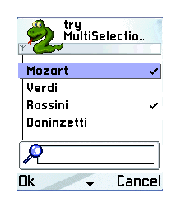
\includegraphics[width=\screenwidth]{markable-list}
\caption{Examples of a checkbox list (left) and a markable list (right)}
\label{fig:checkbox-and-markable-list}
\end{figure}

\subsection{Application Type}
\label{subsec:application}
A single implicit instance of this type always exists when \module{appuifw} 
module is present and can be referred to with the name \code{app}. New 
instances cannot be created by a Python program.

\begin{classdesc*}{Application}
Instances of \class{Application} type have the following attributes:

\begin{memberdesc}[Application]{body}
The UI control that is visible in the application's main window. Currently 
either \class{Text}, a \class{Listbox} object, \class{Canvas}, or 
\code{None}.
\end{memberdesc}

\begin{memberdesc}[Application]{exit_key_handler}
A callable object that is called when the user presses the Exit softkey. 
Setting \member{exit_key_handler} to \code{None} sets it back to the 
default value.
\end{memberdesc}

\begin{memberdesc}[Application]{menu}
This is a list of the following kinds of items:
\begin{itemize}
\item \code{(title, callback)} which creates a regular menu item
\item \code{(title, ((title, callback)\optional{...}))} which creates a submenu
\end{itemize}

\var{title} (Unicode) is the name of the item and \var{callback} the associated callable object. 
The maximum allowed number of items in a menu, or items in a submenu,
or submenus in a menu is 30.

Example:
\begin{verbatim}
appuifw.app.menu = [(u"Item 1", item1),
                    (u"Submenu 1", 
                        ((u"Subitem 1", subitem1),
                         (u"Subitem 2", subitem2)))]
\end{verbatim}
\end{memberdesc}

\begin{memberdesc}[Application]{screen}
The screen area used by an application. See \figurename~\ref{fig:alternate-uilayouts} for
example screens. The appearance of the application on the screen can
be affected by setting one of the following values: \code{'normal'},
\code{'large'}, and \code{'full'}.

Examples:
\begin{verbatim}
appuifw.app.screen='normal' # (a normal screen with title pane and softkeys)
appuifw.app.screen='large'  # (only softkeys visible)
appuifw.app.screen='full'   # (a full screen)
\end{verbatim}
\end{memberdesc}

\begin{memberdesc}[Application]{title}
The title the application that is visible in the application's title
pane. Must be Unicode.
\end{memberdesc}

\begin{memberdesc}[Application]{focus}
A callable object that is called with integer as parameter (0 = focus lost, 
1 = focus regained) when the application receives focus or it is switched to 
background. Focus is received e.g. when the application is switched from 
background to foreground or when the focus is regained from screensaver. 
Similarly when the screensaver is displayed, focus is lost.

Examples:
\begin{verbatim}
>>> import appuifw
>>> def cb(fg):
...   if(fg):
...     print "foreground"
...   else:
...     print "background"
...
>>> appuifw.app.focus=cb
>>> # switch to background, following text is printed from callback:
>>> background
>>> # switch to foreground, following text is printed from callback:
>>> foreground
\end{verbatim}

\begin{notice}
An improper callback can cause adverse effects. If you, for example,
define a callback which takes no parameters you will receive
never-ending \exception{TypeError} exceptions on the Nokia 6600.
\end{notice}

\end{memberdesc}

Instances of \class{Application} type have the following methods:

\begin{methoddesc}[Application]{activate_tab}{index}
Activates the tab \var{index} counting from zero.
\end{methoddesc}

\begin{methoddesc}[Application]{full_name}{}
Returns the full name, in Unicode, of the native application in whose 
context the current Python interpreter session runs.
\end{methoddesc}

\begin{methoddesc}[Application]{set_exit}{}
Requests a graceful exit from the application as soon as the current script 
execution returns.
\end{methoddesc}

\begin{methoddesc}[Application]{set_tabs}{tab_texts\optional{,callback=None}}
Sets tabs with given names on them in the navigation bar; 
\var{tab_texts} is a list of Unicode strings. When the users 
navigate between tabs, \var{callback} gets called with the index 
of the active tab as an argument. Tabs can be disabled by giving an empty or 
one-item \var{tab_texts} list.
\end{methoddesc}

\end{classdesc*}

\subsection{Form Type}
\label{subsec:form}
\class{Form} implements a dynamically configurable, editable multi-field 
dialog. \class{Form} caters for advanced dialog use cases with requirements 
such as free selectability of the combination of fields, possibility of 
validating the user input, and automatically producing the contents of some 
dialog fields before allowing the closing of the dialog. 

\begin{classdesc}{Form}{fields\optional{, flags=0}}
Creates a \class{Form} instance.
\var{fields} is a list of \emph{field descriptors}: \code{(label, type\optional{, value})} where

\var{label} is a Unicode string

\var{type} is one of the following strings: 
\code{'text'}, \code{'number'}, \code{'date'}, \code{'time'}, \code{'combo'}
or \code{'float'}

\var{value}, depending on \var{type}: Unicode string, numeric, float (seconds 
since Unix epoch rounded down to the nearest local midnight), float (seconds 
since local midnight), \code{([choice_label ...], index)} of float. For 
\code{'float'} \var{type} the initial value setting might not be shown in the 
UI.
\end{classdesc}

\class{Form} can also be configured and populated after construction. The 
configuration flags are visible as an attribute. \class{Form} implements 
the list protocol that can be used for setting the form fields, as well as 
obtaining their values after the dialog has been executed.

Instances of \class{Form} type have the following attributes:

\begin{memberdesc}[Form]{flags}
This attribute holds the values of the various configuration flags. 
Currently supported flags are:

\begin{datadesc}{FFormEditModeOnly}
When this flag is set, the form remains in edit mode while \method{execute} 
runs.
\end{datadesc}

\begin{datadesc}{FFormViewModeOnly}
When this flag is set, the form cannot be edited at all.
\end{datadesc}

\begin{datadesc}{FFormAutoLabelEdit}
This flag enables support for allowing the end-users to edit the labels of 
the form fields.
\end{datadesc}

\begin{datadesc}{FFormAutoFormEdit}
This flag enables automatic support for allowing the end-users to add and 
delete the form fields. Note that this is an experimental feature and is not 
guaranteed to work with all SDK versions.
\end{datadesc}

\begin{datadesc}{FFormDoubleSpaced}
When this flag is set, double-spaced layout is applied when the form is 
executed: one field takes two lines, as the label and the value field are on 
different lines.
\end{datadesc}
\end{memberdesc}

\begin{memberdesc}[Form]{menu}
A list of \code{(title, callback)} pairs, where 
each pair describes an item in the form's menu bar that is active while the 
dialog is being executed. \var{title} (Unicode) is the name of 
the item and \var{callback} the associated callable object.
\end{memberdesc}

\begin{memberdesc}[Form]{save_hook}
This attribute can be set to a callable object that receives one argument 
and returns a Boolean value. It gets called every time the users want to 
save the contents of an executing \class{Form} dialog. A candidate list for 
new form content - a list representing the currently visible state of the 
UI - is given as an argument. The list can be modified by 
\member{save_hook}. If \member{save_hook} returns \code{True}, the 
candidate list is set as the new contents of the form. Otherwise, the form 
UI is reset to reflect the field list contained in \class{Form} object.
\end{memberdesc}

Instances of \class{Form} type have the following methods:

\begin{methoddesc}[Form]{execute}{}
Executes the dialog by making it visible on the UI.
\end{methoddesc}

\begin{methoddesc}[Form]{insert}{index, field_descriptor}
Inserts the field descriptor into the \class{Form} before the given \var{index}.
\end{methoddesc}

\begin{methoddesc}[Form]{pop}{}
Removes the last field descriptor from the \class{Form} and returns it.
\end{methoddesc}

\begin{methoddesc}[Form]{length}{}the number of field descriptors in the form.
\end{methoddesc}

The subscript notation \code{f[i]} can be used to access or modify the
i-th element of the form \code{f}. Same limitations as discussed above
in the context of the flag \constant{FFormAutoFormEdit} apply to
modifying a form while it is executing. The ability to change the
schema of a form while it is executing is an experimental feature.

\subsection{Text Type}
\label{subsec:mylabel5}
\class{Text} is a text editor UI control. For examples on the options 
available with \class{Text}, see Figure \ref{fig:text-styles}.

\begin{figure}[htbp]
\centering
\includegraphics[width=\screenwidth]{text-styles-1}
\includegraphics[width=\screenwidth]{text-styles-2}
\caption{Examples of the options available for Text type}
\label{fig:text-styles}
\end{figure}

Instances of \class{Text} type have the following attributes:

\begin{memberdesc}[Text]{color}
The color of the text. \code{color} supports the same color representation 
models as the \module{graphics} module. For the supported color 
representation models, see Section \ref{sec:graphics}.
\end{memberdesc}

\begin{memberdesc}[Text]{focus}
A Boolean attribute that indicates the focus state of the control. Editor 
control also takes the ownership of the navigation bar, and this feature is 
needed to enable the usage of this control in applications that use the 
navigation bar - for example, navigation tabs.
\end{memberdesc}

\begin{memberdesc}[Text]{font} 
The font of the text. There are two possible ways to set this attribute:

\begin{itemize}

\item Using a supported Unicode font, for example \code{u"Latin12"}. Trying to set a font which is not supported by the device has no effect. A list of supported fonts can be retrieved by using \function{appuifw.available_fonts}.

Example, setting font:
\begin{verbatim}
t = appuifw.Text()
t.font = u"albi17b" # sets font to Albi 17 bold
t.font = u"LatinPlain12" # sets font to Latin Plain 12
\end{verbatim}
\item Using one of the default device fonts that are associated with the following labels (plain strings):
\code{'annotation', 'title', 'legend', 'symbol', 'dense', 'normal'}
Example, setting font: 
\begin{verbatim}
t.font = "title" # sets font to the one used in titles
\end{verbatim}

Example, checking the currently set font: 
\begin{verbatim}
unicodeFont = t.font
\end{verbatim}
\end{itemize}

The attribute value retrieved is always a Unicode string. If the font has 
been set with a label, for example, \code{'title'}, the attribute will 
retrieve the font associated with that label. 
\end{memberdesc}

\begin{memberdesc}[Text]{highlight_color}
The highlight color of the text. \code{highlight_color} supports the 
same color representation models as the \module{graphics} module. For the 
supported color representation models, see Section \ref{sec:graphics}.
\end{memberdesc}

\begin{memberdesc}[Text]{style}
The style of the text. The flags for this attribute are defined in the 
\module{appuifw} module. These flags can be combined by using the binary 
operator \code{|}. The flags can be divided into two types: text style 
and text highlight. Text style flags can be freely combined with each other. 
However, one or more text style flags can be combined with only one text 
highlight flag. The flags are:

Text style:

\begin{datadesc}{STYLE_BOLD} 
Enables bold text.
\end{datadesc}

\begin{datadesc}{STYLE_UNDERLINE}
Enables underlined text.
\end{datadesc}

\begin{datadesc}{STYLE_ITALIC} 
Enables italic text.
\end{datadesc}

\begin{datadesc}{STYLE_STRIKETHROUGH } 
Enables strikethrough.
\end{datadesc}

Text highlight:

\begin{datadesc}{HIGHLIGHT_STANDARD}
Enables standard highlight.
\end{datadesc}

\begin{datadesc}{HIGHLIGHT_ROUNDED}
Enables rounded highlight.
\end{datadesc}

\begin{datadesc}{HIGHLIGHT_SHADOW}
Enables shadow highlight.
\end{datadesc}

Only one highlight is allowed to be used at once. Therefore, it is possible 
to combine only one highlight with one or more text styles.

Examples:
\begin{verbatim}
t = appuifw.Text()

# These and other similar values and combinations are valid:
t.style = appuifw.STYLE_BOLD
t.style = appuifw.STYLE_UNDERLINE
t.style = appuifw.STYLE_ITALIC
t.style = appuifw.STYLE_STRIKETHROUGH
t.style = (appuifw.STYLE_BOLD|
	   appuifw.STYLE_ITALIC|
	   appuifw.STYLE_UNDERLINE)

# These values are valid:
t.style = appuifw.HIGHLIGHT_STANDARD
t.style = appuifw.HIGHLIGHT_ROUNDED
t.style = appuifw.HIGHLIGHT_SHADOW

# This combination is NOT valid:
# Invalid code, do not try!
t.style = (appuifw.HIGHLIGHT_SHADOW|appuifw.HIGHLIGHT_ROUNDED)
\end{verbatim}
\end{memberdesc}

Instances of \class{Text} type have the following methods:

\begin{methoddesc}[Text]{add}{text}
Inserts the Unicode string \var{text} to the current cursor position.
\end{methoddesc}

\begin{methoddesc}[Text]{bind}{event_code, callback}
Binds the callable Python object \var{callback} to event
\var{event_code}. The key codes are defined in 
the \module{key_codes} library module. The call 
\code{bind(event_code, None)} clears an 
existing binding. In the current implementation the event is always
passed also to the underlying native UI control.
\end{methoddesc}

\begin{methoddesc}[Text]{clear}{}
Clears the editor.
\end{methoddesc}

\begin{methoddesc}[Text]{delete}{\optional{pos=0, length=len()}}
Deletes \var{length} characters of the text held by the editor control, 
starting from the position \var{pos}.
\end{methoddesc}

\begin{methoddesc}[Text]{get_pos}{}
Returns the current cursor position.
\end{methoddesc}

\begin{methoddesc}[Text]{len}{}
Returns the length of the text string held by the editor control.
\end{methoddesc}

\begin{methoddesc}[Text]{get}{\optional{pos=0, length=len()}}
Retrieves \code{length} characters of the text held by the editor control, 
starting from the position \var{pos}.
\end{methoddesc}

\begin{methoddesc}[Text]{set}{text}
Sets the text content of the editor control to Unicode string 
\var{text}.
\end{methoddesc}

\begin{methoddesc}[Text]{set_pos}{cursor_pos}
Sets the cursor to \var{cursor_pos}.
\end{methoddesc}

\subsection{Listbox Type}
\label{subsec:listbox}

\begin{figure}[htbp]
\centering
\includegraphics[width=\screenwidth]{listbox-with-icons}
\caption{Listbox with icons}
\label{fig:listbox-with-icons}
\end{figure}

An instance of this UI control type is visible as a listbox, also known as a 
list in Symbian, that can be configured to be a single-line item or a 
double-item listbox. Figure \ref{fig:listbox-with-icons} shows a single-line 
item Listbox with icons. For more information on the MBM and MIF formats, 
see Section \ref{subsec:icon}.

\begin{classdesc}{Listbox}{list, callback}
Creates a \class{Listbox} instance. A callable object 
\var{callback} gets called when a listbox selection has been 
made. \code{list} defines the content of the listbox and can be one of the 
following:

\begin{itemize}
\item A normal (single-line item) listbox: a list of Unicode strings, for example \code{[unicode_string item1, unicode_string item2]}
\item A double-item listbox: a two-element tuple of Unicode strings , for example \code{[(unicode_string item1, unicode_string item1description), (unicode_string item2, unicode_string item2description)]}
\item A normal (single-line item) listbox with graphics: a two-element tuple consisting of a Unicode string and an \class{Icon} object, for example \code{[(unicode_string item1, icon1), (unicode_string item2, icon2)]}.
\item A double-item listbox with graphics: a three-element tuple consisting of two Unicode strings and one \class{Icon} object, for example \code{[(unicode_string item1, unicode_string item1description, icon1), (unicode_string item2, unicode_string item2description, icon2)]}
\end{itemize}

Example: To produce a normal (single-line item) listbox with graphics:
\begin{verbatim}
icon1 = appuifw.Icon(u"z:\\system\\data\\avkon.mbm", 28, 29)
icon2 = appuifw.Icon(u"z:\\system\\data\\avkon.mbm", 40, 41)
entries = [(u"Signal", icon1),
           (u"Battery", icon2)]
lb = appuifw.Listbox(entries, lbox_observe)
\end{verbatim}
\end{classdesc}

Instances of \class{Listbox} type have the following methods:

\begin{methoddesc}[Listbox]{bind}{event_code, callback}
Binds the callable Python object \var{callback} to event 
\var{event_code}. The key codes are defined in 
the \module{key_codes} library module. The call
\code{bind(event_code, None)} clears an 
existing binding. In the current implementation the event is always passed 
also to the underlying native UI control.
\end{methoddesc}

\begin{methoddesc}[Listbox]{current}{}
Returns the currently selected item's index in the \class{Listbox}.
\end{methoddesc}

\begin{methoddesc}[Listbox]{set_list}{list\optional{, current}}
Sets the \class{Listbox} content to a list of Unicode strings or a
list of tuples of Unicode strings. The accepted structures of \var{list} are the
same as in the \class{Listbox} constructor. The optional argument \var{current} is the index of the focused list item.
\end{methoddesc}

\subsection{Icon Type}
\label{subsec:icon}
An instance of \class{Icon} type encapsulates an icon to be used together 
with a \class{Listbox} instance. Note that currently \class{Icon} can only 
be used with \class{Listbox} (see Section \ref{subsec:listbox}).

MBM is the native Symbian OS format used for pictures. It is a
compressed file format where the files can contain several bitmaps and
can be referred to by a number. An \code{.mbg} file is the header file
usually associated with an \code{.mbm} file, which includes symbolic
definitions for each bitmap in the file. For example, an
\file{avkon.mbm} file has an associated index file called
\file{avkon.mbg}, which is included in S60 SDKs. For more information
on the MBM format and the bitmap converter tool, see \cite{S60Doc} and
search the topics with the key term "How to provide Icons"; this topic
also points you to the Bitmap Converter tool that can be used for
converting bitmaps into the MBM format.

S60 2$^{nd}$ Edition FP3 introduces a new format for icons called 
Multi-Image File (MIF). This format is very similar to the MBM format and 
also contains several compressed files. The files to be compressed should be 
in Scalable Vector Graphics Tiny (SVG-T) format. For more information on the 
SVG format, see Scalable Vector Graphics (SVG) 1.1 Specification 
[10].

\begin{classdesc}{Icon}{filename, bitmap, bitmapMask}
Creates an icon. \var{filename} is a Unicode file name and must 
include the whole path. Note that MBM and MIF (MIF only in S60 2nd 
Edition FP3) are the only file formats supported. \var{bitmap} 
and \var{bitmapMask} are integers that represent the index of 
the icon and icon mask inside that file respectively.
\end{classdesc}

Example: The following builds an icon with the standard signal symbol:
\begin{verbatim}
icon = appuifw.Icon(u"z:\\system\\data\\avkon.mbm", 28, 29)
\end{verbatim}

\subsection{Content_handler Type}
\label{subsec:content}

An instance of \class{Content_handler} handles data content by its MIME 
type.

\begin{classdesc}{Content_handler}{\optional{callback}}
Creates a \class{Content_handler} instance. A Content_handler handles
data content by its MIME type. The optional
\var{callback} is called when the embedded handler application 
started with the \method{open} method finishes. 
\end{classdesc}

Instances of \class{Content_handler} type have the following methods:

\begin{methoddesc}[Content_handler]{open}{filename}
Opens the file \var{filename} (Unicode) in its handler 
application if one has been registered for the particular MIME type. The 
handler application is embedded in the caller's thread. The call to this 
function returns immediately. When the handler application finishes, the 
\var{callback} that was given to the \class{Content_handler} 
constructor is called.
\end{methoddesc}

\begin{methoddesc}[Content_handler]{open_standalone}{filename}
Opens the file \var{filename} (Unicode) in its handler 
application if one has been registered for the particular MIME type. The 
handler application is started in its own process. The call to this function 
returns immediately. Note that \var{callback} is not called for 
applications started with this method.
\end{methoddesc}

\subsection{Canvas Type}
\label{subsec:canvas}
\class{Canvas} is a UI control that provides a drawable area on the screen 
and support for handling raw key events. \class{Canvas} supports the 
standard drawing methods that are documented in Section \ref{sec:graphics}.

\begin{classdesc}{Canvas}{\optional{redraw_callback=None, event_callback=None}}
Constructs a \class{Canvas}. The optional parameters are callbacks
that are called when specific events occur. 

\note{Watch out for cyclic
references here. For example, if the callbacks are methods of an
object that holds a reference to the \class{Canvas}, a reference cycle
is formed that must be broken at cleanup time or the
\class{Canvas} will not be freed.}

\var{redraw_callback} is called whenever a part of the \class{Canvas} 
has been obscured by something, is then revealed, and needs to be
redrawn. This can typically happen, for example, when the user
switches away from the Python application and back again, or after
displaying a pop-up menu. The callback takes as its argument a
four-element tuple that contains the top-left and the bottom-right
corner of the area that needs to be redrawn. In many cases redrawing
the whole
\class{Canvas} is a reasonable option. 

\var{event_callback} is called whenever a raw key event is received.
There are three kinds of key events: \code{EEventKeyDown},
\code{EEventKey}, and \code{EEventKeyUp}. When a user presses a key 
down, events \code{EEventKeyDown} and \code{EEventKey} are generated. 
When the key is released, an \code{EEventKeyUp} event is generated.

The argument to the \var{event_callback} is a dictionary that contains 
the following data for key events:

\begin{itemize}
\item \code{'type'}: one of \code{EEventKeyDown}, \code{EEventKey}, or \code{EEventKeyUp}
\item \code{'keycode'}: the keycode of the key
\item \code{'scancode'}: the scancode of the key
\item \code{'modifiers'}: the modifiers that apply to this key event
\end{itemize}

Each key on the keyboard has one or more scancodes and zero or more keycodes 
associated with it. A scancode represents the physical key itself and a 
keycode is the result of state-related operating system defined processing 
done on the key. For keys that correspond to a symbol in the current 
character set of the phone, the keycode is equal to the code of the 
corresponding symbol in that character set. For example, if you are using 
the Nokia Wireless Keyboard (SU-8W), pressing the key A will always produce 
the scancode 65 (ASCII code for an upper case A), but the keycode 
could be either 65 or 91 (ASCII code for a lower case A) depending on 
whether or not the Shift key is pressed or Caps Lock is active. 

The \module{key_codes} module contains definitions for the keycodes and 
scancodes. See \figurename~\ref{fig:keyboard} for the codes of the most 
common keys on the phone keypad. 

Some keys are handled in a special way:

\begin{itemize}
\item A short press of the Edit key causes it to stay down, meaning that no \code{EEventKeyUp} event is sent. The event is only sent after a long press.
\item Detecting presses of the Voice tags key or the Power key is not supported.
\item If the right softkey is pressed, the \code{appuifw.app.exit_key_handler} callback is always executed.
\end{itemize}

There is no way to prevent the standard action of the Hang-up key, the Menu 
key, the Power key or the Voice tags key from taking place.

\begin{figure}
\centering
\includegraphics[width=5in]{6630keyboard}
%\includegraphics[width=3.60in,height=2.58in]{6630keyboard}
%\centerline{\includegraphics[width=3.60in,height=2.58in]{API_Reference_for_Python11.eps}} \par & 
\begin{tableiii}{lll}{textrm}{Key}{Keycode}{Scancode}
\lineiii{1.}{EKeyLeftSoftkey}{EScancodeLeftSoftkey}
\lineiii{2.}{EKeyYes}{EScancodeYes}
\lineiii{3.}{EKeyMenu}{EScancodeMenu}
\lineiii{4.}{EKey0...9}{EScancode0...9}
\lineiii{5.}{EKeyStar}{EScancodeStar}
\lineiii{6.}{EKeyLeftArrow}{EScancodeLeftArrow}
\lineiii{7.}{EKeyUpArrow}{EScancodeUpArrow}
\lineiii{8.}{EKeySelect}{EScancodeSelect}
\lineiii{9.}{EKeyRightArrow}{EScancodeRightArrow}
\lineiii{10.}{EKeyDownArrow}{EScancodeDownArrow}
\lineiii{11.}{EKeyRightSoftkey}{EScancodeRightSoftkey}
\lineiii{12.}{EKeyNo}{EScancodeNo}
\lineiii{13.}{EKeyBackspace}{EScancodeBackspace}
\lineiii{14.}{EKeyEdit}{EScancodeEdit}
\lineiii{15.}{EKeyHash}{EScancodeHash}
\end{tableiii}
\caption{Keycodes and scancodes for phone keys usable from Python applications}
\label{fig:keyboard}
\end{figure}

\end{classdesc}

Instances of \class{Canvas} type have the following attribute:

\begin{memberdesc}[Canvas]{size}
A two-element tuple that contains the current width and height of the 
\class{Canvas} as integers.
\end{memberdesc}

Instances of \class{Canvas} type have the same standard drawing methods 
that are documented in Section \ref{sec:graphics}.

\input{libgraphics}
% Copyright (c) 2005 Nokia Corporation
%
% Licensed under the Apache License, Version 2.0 (the "License");
% you may not use this file except in compliance with the License.
% You may obtain a copy of the License at
%
%     http://www.apache.org/licenses/LICENSE-2.0
%
% Unless required by applicable law or agreed to in writing, software
% distributed under the License is distributed on an "AS IS" BASIS,
% WITHOUT WARRANTIES OR CONDITIONS OF ANY KIND, either express or implied.
% See the License for the specific language governing permissions and
% limitations under the License.

\section{\module{camera} ---
    Interface for taking photographs}

\declaremodule{extension}{camera}
\label{sec:camera}

\begin{notice}[note]
Not available for S60 1st Edition.
\end{notice}

The \module{camera} module enables taking photographs. 

The \module{camera} module has the following functions\footnote{ 
Descriptions for some of the values are based on information found in S60 SDK documentation \cite{S60Doc}}:

\begin{funcdesc}{cameras_available}{}
Returns the number of cameras available in the device.
\end{funcdesc}

\begin{funcdesc}{image_modes}{}
Returns the image modes supported in the device as a list of strings, for 
example: \code{['RGB12', 'RGB', 'RGB16'].}
\end{funcdesc}

\begin{funcdesc}{image_sizes}{}
Returns the image sizes (resolution) supported in the device as a list of 
\code{(x, y)} tuples, for example: \code{[(640, 480), (160, 120)]}.
\end{funcdesc}

\begin{funcdesc}{flash_modes}{}
Returns the flash modes available in the device as a list of strings. 
\end{funcdesc}

\begin{funcdesc}{max_zoom}{}
Returns the maximum digital zoom value supported in the device as an 
integer. 
\end{funcdesc}

\begin{funcdesc}{exposure_modes}{}
Returns the exposure settings supported in the device as a list of strings. 
\end{funcdesc}

\begin{funcdesc}{white_balance_modes}{}
Returns the white balance modes available in the device as a list of 
strings. 
\end{funcdesc}

\begin{funcdesc}{take_photo}{\optional{mode, size, flash, zoom, exposure, white_balance, position}}
Takes a photograph and returns the image in \code{Image} format (for more 
information on \code{Image} format, see Chapter \ref{sec:graphics} 
\refmodule{graphics} Module). If some other application is using the camera, 
this operation fails, for example with \code{SymbianError: KErrInUse}. The 
settings listed below describe all settings that are supported by the 
\code{camera} module. You can retrieve the mode settings available for your 
device by using the appropriate functions listed at the beginning of this 
chapter.

\begin{itemize}
\item \var{mode} is the display mode of the image. The default value is \code{'RGB16'}. The following display modes are supported:
	\begin{itemize}
	\item \code{'RGB12'}: 4096 colors (12 bits per pixel)
	\item \code{'RGB16'}: 65536 colors (16 bits per pixel). Default value, always supported
	\item \code{'RGB'}: 16.7 million colors (24 bits per pixel)
	\end{itemize}
\item \var{size} is the resolution of the image. The default value is \code{(640, 480)}. The following sizes are supported, for example, in Nokia 6630: \code{(1280, 960)}, \code{(640, 480)} and \code{(160, 120)}.
\item \var{flash} is the flash mode setting. The default value is \code{'none'}. The following flash mode settings are supported:
	\begin{itemize}
	\item \code{'none' \newline
}No flash. Default value, always supported
	\item \code{'auto' \newline
}Flash will automatically fire when required
	\item \code{'forced' \newline
}Flash will always fire
	\item \code{'fill_in' \newline
}Reduced flash for general lighting
	\item \code{'red_eye_reduce' \newline
}Red-eye reduction mode
	\end{itemize}
\item \var{zoom} is the digital zoom factor. It is assumed to be on a linear scale from 0 to the maximum zoom value allowed in the device. The default value is \code{0}, meaning that zoom is not used. 
\item \var{exposure} is the exposure adjustment of the device. Exposure is a combination of lens aperture and shutter speed used in taking a photograph. The default value is \code{'auto'.} The following exposure modes are supported:
	\begin{itemize}
	\item \code{'auto'} \newline
Sets exposure automatically. Default value, always supported
	\item \code{'night'} \newline
Night-time setting for long exposures
	\item \code{'backlight' } \newline
Backlight setting for bright backgrounds
	\item \code{'center'} \newline
Centered mode for ignoring surroundings
	\end{itemize}
\item \var{white_balance} can be used to adjust white balance to match the main source of light. The term white balance refers to the color temperature of the current light. A digital camera requires a reference point to represent white. It will then calculate all the other colors based on this white point. The default value for \var{white_balance} is \code{'auto'} and the following white balance modes are supported:
	\begin{itemize}
	\item \code{'auto'} \newline
Sets white balance automatically. Default value, always supported
	\item \code{'daylight'} \newline
Sets white balance to normal daylight
	\item \code{'cloudy}' \newline
Sets white balance to overcast daylight
	\item \code{'tungsten'} \newline
Sets white balance to tungsten filament lighting
	\item \code{'fluorescent}' \newline
Sets white balance to fluorescent tube lighting
	\item \code{'flash'} \newline
Sets white balance to flash lighting
	\end{itemize}
\item \var{position} is the camera used if the device, such as Nokia 6680, has several cameras. In Nokia 6680, the camera pointing to the user of the device is located in position \code{1}, whereas the one pointing away from the user is located in position \code{0}. The default \var{position} is \code{0}.
\end{itemize}
\end{funcdesc}


\chapter{Audio and Communication Services \label{s60ac}}

\input{libaudio}
% Copyright (c) 2005 Nokia Corporation
%
% Licensed under the Apache License, Version 2.0 (the "License");
% you may not use this file except in compliance with the License.
% You may obtain a copy of the License at
%
%     http://www.apache.org/licenses/LICENSE-2.0
%
% Unless required by applicable law or agreed to in writing, software
% distributed under the License is distributed on an "AS IS" BASIS,
% WITHOUT WARRANTIES OR CONDITIONS OF ANY KIND, either express or implied.
% See the License for the specific language governing permissions and
% limitations under the License.

\section{\module{telephone} ---
	 Telephone services}
\label{sec:telephone}

\declaremodule{extension}{telephone}
\platform{S60}
\modulesynopsis{A telephone related services package.}

This module provides an API to a telephone. 

Since the users of the device can also hang-up the phone explicitly, they 
might affect the current status of the call. In addition, using this 
extension in an emulator has no effect since no calls can be connected.

The \module{telephone} module has the following functions:

\begin{funcdesc}{dial}{number}

Dials the number set in \var{number}. \var{number} 
is a string, for example \code{u'+358501234567'} where \code{'+'} is the 
international prefix, \code{'358'} is the country code, \code{'50'} is 
the mobile network code (or the area code), and \code{'1234567'} is the 
subscriber number. If there is an ongoing phone call prior to calling 
\method{dial} from Python, then the earlier call is put on hold and a new 
call is established. Calling \method{dial} multiple times when, for example, 
the first call has been answered and a line has been established results in 
subsequent calls not being connected.
\end{funcdesc}

\begin{funcdesc}{hang\_up}{}
Hangs up if a call initiated by \method{dial} is in process. If this call 
has already been finished, \exception{SymbianError: KErrNotReady} is raised.
\end{funcdesc}

\input{libmessaging}
\input{libinbox}
\input{liblocation}

\chapter{Data Management \label{s60data}}

\input{libcontacts}
\input{libcalendar}
\input{libe32db}
\input{libe32dbm}

\chapter{Standard Library Support and Extensions \label{s60lib}}

% Copyright (c) 2005 Nokia Corporation
%
% Licensed under the Apache License, Version 2.0 (the "License");
% you may not use this file except in compliance with the License.
% You may obtain a copy of the License at
%
%     http://www.apache.org/licenses/LICENSE-2.0
%
% Unless required by applicable law or agreed to in writing, software
% distributed under the License is distributed on an "AS IS" BASIS,
% WITHOUT WARRANTIES OR CONDITIONS OF ANY KIND, either express or implied.
% See the License for the specific language governing permissions and
% limitations under the License.

\section{Support for Python Standard Library}
\label{sec:standard}

The standard library support in Python for S60 is summarized in Table 
\ref{standardsupport}. For API descriptions, see \cite{PyLibRef}.

\begin{center}
\begin{longtable}{|l|l|l|p{200pt}|}
\hline
{\bf Name}& 
{\bf Type}& 
{\bf Status}& 
{\bf Remarks} \\
\hline
\code{{\_}testcapi}& 
PYD& 
Y& 
 \\
\hline
\code{anydbm}& 
PY& 
X& 
DBM API is implemented by PY \code{e32dbm} that relies on PYD \code{e32db} (see Chapter \ref{sec:e32dbm}, e32dbm Module) \\
\hline
\code{atexit}& 
PY& 
X& 
 \\
\hline
\code{base64}& 
PY& 
X& 
 \\
\hline
\code{bdb}& 
PY& 
(X)& 
 \\
\hline
\code{binascii}& 
built-in& 
X& 
 \\
\hline
\code{cmd}& 
PY& 
(X)& 
 \\
\hline
\code{code}& 
PY& 
X& 
 \\
\hline
\code{codecs}& 
PY& 
X& 
 \\
\hline
\code{codeop}& 
PY& 
X& 
 \\
\hline
\code{copy}& 
PY& 
X& 
 \\
\hline
\code{copy{\_}reg}& 
PY& 
X& 
 \\
\hline
\code{cStringIO}& 
built-in& 
X& 
 \\
\hline
\code{dis}& 
PY& 
(X)& 
 \\
\hline
\code{errno}& 
built-in& 
X& 
 \\
\hline
\code{exceptions}& 
built-in& 
X& 
 \\
\hline
\code{{\_}{\_}future{\_}{\_}}& 
PY& 
X& 
 \\
\hline
\code{httplib}& 
PY& 
X& 
 \\
\hline
\code{imp}& 
built-in& 
X& 
 \\
\hline
\code{keyword}& 
PY& 
X& 
 \\
\hline
\code{linecache}& 
PY& 
X& 
 \\
\hline
\code{marshal}& 
built-in& 
X& 
 \\
\hline
\code{math}& 
built-in& 
X& 
 \\
\hline
\code{md5}\footnote{Derived from the RSA Data Security, Inc. MD5 Message-Digest Algorithm.}& 
built-in& 
X& 
 \\
\hline
\code{mimetools}& 
PY& 
X& 
 \\
\hline
\code{operator}& 
built-in& 
X& 
 \\
\hline
\code{os, os.path}& 
PY& 
X& 
Wraps built-in \code{e32posix}. Limitations discussed in Section \ref{subsec:limitations}, Limitations and Areas of Development. \\
\hline
\code{pdb}& 
PY& 
(X)& 
 \\
\hline
\code{quopri}& 
PY& 
X& 
 \\
\hline
Name& 
Type& 
Status& 
Remarks \\
\hline
\code{random}& 
PY& 
X& 
 \\
\hline
\code{re}& 
PY& 
X& 
Uses PY \code{sre} as its engine. \\
\hline
\code{repr}& 
PY& 
X& 
 \\
\hline
\code{rfc822}& 
PY& 
X& 
 \\
\hline
\code{select}& 
PY& 
X& 
A minimal implementation: \code{select} is supported only for input from sockets. \\
\hline
\code{socket}& 
PY& 
X& 
Requires PYD \code{e32socket}. Contains extensions as described in Section \ref{subsec:socket}, socket Module. Limitations discussed in Section \ref{subsec:limitations}, Limitations and Areas of Development.  \\
\hline
\code{sre}& 
PY& 
X& 
Wraps built-in \code{{\_}sre}. \\
\hline
\code{string}& 
PY& 
X& 
 \\
\hline
\code{StringIO}& 
PY& 
X& 
 \\
\hline
\code{struct}& 
built-in& 
X& 
 \\
\hline
\code{sys}& 
built-in& 
X& 
 \\
\hline
\code{thread}& 
built-in& 
X& 
Contains extensions as described in Section \ref{subsec:thread}, thread Module \\
\hline
\code{threading}& 
PY& 
(X)& 
 \\
\hline
\code{time}& 
built-in& 
X& 
 \\
\hline
\code{traceback}& 
PY& 
X& 
 \\
\hline
\code{types}& 
PY& 
X& 
 \\
\hline
\code{urllib}& 
PY& 
X& 
 \\
\hline
\code{urlparse}(urlsplit only)& 
PY& 
X& 
 \\
\hline
\code{uu}& 
PY& 
X& 
 \\
\hline
\code{warnings}& 
PY& 
X& 
 \\
\hline
\code{whichdb}& 
PY& 
X& 
 \\
\hline
\code{xreadlines}& 
built-in& 
X& 
 \\
\hline
\code{zipfile}& 
PY& 
X& 
 \\
\hline
\code{zlib}& 
PYD& 
X& 
 \\
\hline
\caption{Status of library module support.}
\label{standardsupport}
\end{longtable}
\end{center}

Table \ref{standardsupport} uses the following coding for module types:

\begin{itemize}
\item PY -- module is implemented in Python.
\item Built-in -- module is a built-in C/C++ module.
\item PYD -- module is a dynamically loadable C/C++ module.
\end{itemize}
For support status, the following codes are used:

\begin{enumerate}
\item[\textbullet] X -- included to the Series 60 Python distribution.
\item[\textbullet] (X) -- not included to the Series 60 Python distribution, but works both on phone and SDK.
\item[\textbullet] Y -- included only to the SDK distribution.
\end{enumerate}


\section{Extensions to Standard Library Modules}
\label{extensions}

The following standard modules have been extended.

\subsection{\module{thread} ---
  S60 extensions to standard thread module} 
\label{subsec:thread}

\declaremodule{extension}{thread}
\modulesynopsis{S60 extensions to standard thread module.}

The following function has been added to the standard \code{thread} 
module:

\begin{funcdesc}{ao_waittid}{thread_id}

Synchronizes with the end of the execution of the thread identified by the given 
\var{thread_id}. The implementation is based on a Symbian OS active object. 
For the blocking behavior, see Section \ref{subsec:Aolock}, Ao_lock Type.

\end{funcdesc}

\subsection{\module{socket} ---
  S60 extensions to standard socket module} 
\label{subsec:socket}

\declaremodule{extension}{socket}
\modulesynopsis{Extensions to standard socket module.}

Bluetooth (BT) support has been added to the standard \code{socket} 
module. The following related constants and functions are defined:

\begin{notice}[note]
In release 1.0 the functions \code{bt_advertise_service}, 
\code{bt_obex_receive}, and 
\code{bt_rfcomm_get_available_server_channel} incorrectly 
expected to be given the internal \code{e32socket.socket} object as the 
socket parameter instead of the proper \code{socket} object. Now the 
functions work correctly. The old calling convention is still supported but 
it is deprecated and may be removed in a future release.
\end{notice}

\begin{datadesc}{AF_BT}

Represents the Bluetooth address family.

\end{datadesc}

\begin{datadesc}{BTPROTO_RFCOMM}

This constant represents the Bluetooth protocol RFCOMM.

\end{datadesc}

\begin{datadesc}{RFCOMM}
\end{datadesc}
\begin{datadesc}{OBEX}

Bluetooth service classes supported by \code{bt_advertise_service}.

\end{datadesc}

\begin{datadesc}{AUTH}
\end{datadesc}
\begin{datadesc}{ENCRYPT}
\end{datadesc}
\begin{datadesc}{AUTHOR}

Bluetooth security mode flags.

\end{datadesc}

\begin{funcdesc}{bt_advertise_service}{name, socket, flag, class}

Sets a service advertising the service \var{name} (Unicode) on local channel 
that is bound to \var{socket}. If \var{flag} is \code{True}, the advertising is 
turned on, otherwise it is turned off. The service class to be advertised is 
either \code{RFCOMM} or \code{OBEX}.

\end{funcdesc}

\begin{funcdesc}{bt_discover}{\optional{address}}

Performs the Bluetooth device discovery (if the optional BT device address 
is not given) and the discovery of RFCOMM class services on the chosen 
device. Returns a pair: BT device address, dictionary of services, where 
Unicode service name is the key and the corresponding port is the value.

\end{funcdesc}

\begin{funcdesc}{bt_obex_discover}{\optional{address}}

Same as \code{discover}, but for discovery of OBEX class services on the 
chosen device.

\end{funcdesc}

\begin{funcdesc}{bt_obex_send_file}{address, channel, filename}

Sends file \var{filename} (Unicode) wrapped into an OBEX object 
to remote \var{address}, \var{channel}.

\end{funcdesc}

\begin{funcdesc}{bt_obex_receive}{socket, filename}

Receives a file as an OBEX object, unwraps and stores it into \var{filename} 
(Unicode). \var{socket} is a bound \code{OBEX} socket.

\end{funcdesc}

\begin{funcdesc}{bt_rfcomm_get_available_server_channel}{socket}

Returns an available RFCOMM server channel for \var{socket}.

\end{funcdesc}

\begin{funcdesc}{set_security}{socket, mode}

Sets the security level of the given bound \var{socket}. The 
\var{mode} is an integer flag that is formed using a binary 
\code{or} operation of one or more of: \code{AUTH} (authentication), 
\code{ENCRYPT}, \code{AUTHOR} (authorization). Example: 
\code{set_security(s, AUTH | AUTHOR)}.

\end{funcdesc}

\begin{notice}[note]
When listening to a Bluetooth socket on the phone, it is necessary to set 
the security level.
\end{notice}

\begin{notice}[note]
SSL is not supported in S60 1st Edition. SSL client certificates are 
not supported at all.
\end{notice}

For examples on the usage of these functions, see Programming with Python for 
S60 Platform \cite{PyS60Prog}.


\chapter{Extending and Embedding \label{s60ext}}

\input{capiextensions}
\input{extending}

\input{libabbreviations}
\input{libreferences}

\appendix

\chapter{Reporting Bugs}
\input{reportingbugs}


%  The ugly "%begin{latexonly}" pseudo-environments are really just to
%  keep LaTeX2HTML quiet during the \renewcommand{} macros; they're
%  not really valuable.


%begin{latexonly}
\renewcommand{\indexname}{Module Index}
%end{latexonly}
\input{modlib.ind}              % Module Index

%begin{latexonly}
\renewcommand{\indexname}{Index}
%end{latexonly}
% Portions Copyright (c) 2005 Nokia Corporation
\documentclass{manual}

% NOTE: this file controls which chapters/sections of the library
% manual are actually printed.  It is easy to customize your manual
% by commenting out sections that you're not interested in.

\title{PyS60 Library Reference}

\input{boilerplate}

\makeindex                      % tell \index to actually write the
                                % .idx file
\makemodindex                   % ... and the module index as well.

%begin{latexonly}
\ifx\pdftexversion\undefined
 \usepackage[dvips]{graphicx}
\else
 \usepackage[pdftex]{graphicx}
\fi
%end{latexonly}
\usepackage{graphicx}

\usepackage{longtable}

\graphicspath{{./}{figures/}}

\begin{document}

\maketitle

\ifhtml
\chapter*{Front Matter\label{front}}
\fi

\input{copyright}

\begin{abstract}

\noindent

The Python for S60 Platform (Python for S60) simplifies application development 
and provides a scripting solution for the Symbian C++ APIs. This document is for 
Python for S60 version \productversion that is based on Python 2.2.2.

\end{abstract}

\tableofcontents

                                % Chapter title:

% Copyright (c) 2005 Nokia Corporation
%
% Licensed under the Apache License, Version 2.0 (the "License");
% you may not use this file except in compliance with the License.
% You may obtain a copy of the License at
%
%     http://www.apache.org/licenses/LICENSE-2.0
%
% Unless required by applicable law or agreed to in writing, software
% distributed under the License is distributed on an "AS IS" BASIS,
% WITHOUT WARRANTIES OR CONDITIONS OF ANY KIND, either express or implied.
% See the License for the specific language governing permissions and
% limitations under the License.

\chapter{Introduction}
\label{intro}

% XXX add macro version here
The Python for S60 Platform (Python for S60) simplifies 
application development and provides a scripting solution for the Symbian 
C++ APIs. This document is for Python for S60 release 1.3.1 that is 
based on Python 2.2.2.

The documentation for Python for S60 includes three documents:

\begin{itemize}
\item Getting Started with Python for S60 Platform \cite{PyS60Start} contains information on how to install Python for S60 and how to write your first program.
\item This document contains API and other reference material.
\item Programming with Python for S60 Platform \cite{PyS60Prog} contains code examples and programming patterns for S60 devices that can be used as a basis for programs.
\end{itemize}
Python for S60 as installed on a S60 device consists of:

\begin{itemize}
\item Python execution environment, which is visible in the application menu of the device and has been written in Python on top of Python for S60 Platform (see S60 SDK documentation \cite{S60Doc})
\item Python interpreter DLL
\item Standard and proprietary Python library modules
\item S60 UI application framework adaptation component (a DLL) that connects the scripting domain components to the S60 UI
\item Python Installer program for installing Python files on the device, which consists of:
	\begin{itemize}
	\item Recognizer plug-in
	\item Symbian application written in Python
	\end{itemize}
\end{itemize}

The Python for S60 developer discussion board \cite{PyS60DiBo} on the 
Forum Nokia Web site is a useful resource for finding out information on 
specific topics concerning Python for S60. You are welcome to give 
feedback or ask questions about Python for S60 through this discussion 
board.

\section{Scope}
\label{subsec:scope}

This document includes the information required by developers to create 
applications that use Python for S60, and some advice on extending the 
platform.

\section{Audience}
\label{subsec:audience}

This guide is intended for developers looking to create programs that use the 
native features and resources of the S60 phones. The reader should be 
familiar with the Python programming language (\url{http://www.python.org/}) and 
the basics of using Python for S60 (see Getting Started with Python for 
S60 Platform \cite{PyS60Start}).

% XXX version macro to this declaration
\section{New in Release 1.3.1}
\label{subsec:new}

% XXX macro could include version-1 also
This section lists the updates in this document since release 1.2.

\begin{itemize}
\item New attribute \code{focus}, \ref{subsec:application}, Application Type.
\item Support for float values in \code{query} and \code{Form}, \ref{subsec:module}, Module Level Functions and \ref{subsec:form}, Form Type respectively.
\item Global note in \code{note}, \ref{subsec:module}, Module Level Functions.
\item Setting the device time, \ref{subsec:e32}, Module Level Functions.
\item New type \code{Ao_timer}, \ref{subsec:Aotimer}, Ao\_timer Type.
\item Section \ref{sec:inbox}, \code{inbox} Module has been added.
\item New functionality in \code{Sound}, \ref{subsec:sound}, Sound Objects.
\end{itemize}

\section{Naming Conventions}
\label{subsec:naming}

Most names of the type \code{ESomething} typically indicate a constant defined 
by the Symbian SDK. More information about these constants can be found in the 
Symbian SDK documentation.
                % Introduction

% Copyright (c) 2005 Nokia Corporation
%
% Licensed under the Apache License, Version 2.0 (the "License");
% you may not use this file except in compliance with the License.
% You may obtain a copy of the License at
%
%     http://www.apache.org/licenses/LICENSE-2.0
%
% Unless required by applicable law or agreed to in writing, software
% distributed under the License is distributed on an "AS IS" BASIS,
% WITHOUT WARRANTIES OR CONDITIONS OF ANY KIND, either express or implied.
% See the License for the specific language governing permissions and
% limitations under the License.

\chapter{API Summary}
\label{sec:summary}

All built-in object types of the Python language are supported in the
S60 environment. The rest of the programming interfaces are
implemented by various library modules as summarized in this chapter.

\section{Python Standard Library}
\label{subsec:python}

% XXX appendix reference
Python for S60 platform distribution does not include all of the 
Python's standard and optional library modules to save storage space in the 
phone. Nevertheless, many of the excluded modules also work in the S60 
Python environment without any modifications. Some modules are included in 
the SDK version but not installed in the phone. For a summary of supported 
library modules, see Chapter \ref{s60lib}.

When Python, available at \url{http://www.python.org/}, is installed on a PC, the 
library modules are by edefault located in \file{\textbackslash Python22\textbackslash Lib}
on Windows and in \file{/usr/lib/python2.2} on Linux. The Python library 
modules' APIs are documented in \cite{PyLibRef}.

Python for S60 extends some standard modules. These extensions are 
described in this document, see Chapter \ref{extensions}.

\section{Python for S60 Extensions}
\label{sec:sumext}

There are two kinds of native C++ extensions in the Python for S60 
Platform: built-in extensions and dynamically loadable extensions.

\subsection{Built-in extensions}
\label{sec:built}

There are two built-in extensions in the Python for S60 package:

\begin{itemize}
\item The \refmodule{e32} extension module is built into the Python interpreter on Symbian OS, and implements interfaces to special Symbian OS Platform services that are not accessible via Python standard library modules.
\item The \refmodule{appuifw} module for Python for S60 Platform offers UI application framework related Python interfaces.
\end{itemize}

\subsection{Dynamically loadable extensions}
\label{sec:dynamically}

These dynamically loadable extension modules provide proprietary APIs
to S60 Platform's services: \refmodule{graphics} (see Chapter
\ref{sec:graphics}, graphics Module), \refmodule{e32db} (see Chapter
\ref{sec:e32db}, e32db Module),
\refmodule{messaging} (see Chapter \ref{sec:messaging}, messaging Module), 
\refmodule{inbox} (see Chapter \ref{sec:inbox}, inbox Module), \refmodule{location} 
(see Chapter \ref{sec:location}, location Module), \refmodule{sysinfo} (see Chapter 
\ref{sec:sysinfo}, sysinfo Module), \refmodule{camera} (see Chapter 
\ref{sec:camera}, camera Module), \refmodule{audio} (see Chapter \ref{sec:audio}, 
audio Module), \refmodule{telephone} (see Chapter \ref{sec:telephone}, telephone 
Module), \refmodule{calendar} (see Chapter \ref{sec:calendar}, calendar Module), 
and \refmodule{contacts }(see Chapter \ref{sec:contacts}, contacts Module).

\section{Third-Party Extensions}
\label{subsec:third}

% XXX appendix references
It is also possible to write your own Python extensions. S60 related
extensions to Python/C API are described in Chapter
\ref{capiextensions}. For some further guidelines on writing
extensions in C/C++, see Chapter \ref{extending}. In
addition, for an example on porting a simple extension to S60, see
\cite{PyS60Prog}.
              % API summary

% Copyright (c) 2005 Nokia Corporation
%
% Licensed under the Apache License, Version 2.0 (the "License");
% you may not use this file except in compliance with the License.
% You may obtain a copy of the License at
%
%     http://www.apache.org/licenses/LICENSE-2.0
%
% Unless required by applicable law or agreed to in writing, software
% distributed under the License is distributed on an "AS IS" BASIS,
% WITHOUT WARRANTIES OR CONDITIONS OF ANY KIND, either express or implied.
% See the License for the specific language governing permissions and
% limitations under the License.

\chapter{Selected Issues on Python Programming for S60}
\label{sec:selected}

The following issues must be considered when using Python on S60.

\section{Concurrency Aspects}
\label{subsec:concurrency}
The thread that initializes the Python interpreter becomes the main Python 
thread. This is usually the main thread of a UI application. When an 
application written in Python launches, the Symbian platform infrastructure 
creates the main UI thread that starts the Python environment. If a Python 
program is started as a server with \code{e32.start_server}, then the 
Python main thread is not a UI thread.

It is possible to launch new threads via the services of \module{thread} 
module. Examples of such situations could be to overcome eventual problems 
with the fixed, relatively small stack size of the main UI application 
thread; or to perform some background processing while still keeping the UI 
responsive. These new threads are not allowed to directly manipulate the UI; 
in other words, they may not use the \module{appuifw} module.

Because of the limitations of the Python interpreter's final cleanup, Python 
applications on the Symbian OS should be designed in such a way that the 
main thread is the last thread alive.

A facility called active object is used extensively on the Symbian OS to 
implement co-operative, non-preemptive scheduling within operating system 
threads. This facility is also utilized with native APIs. A Python 
programmer is exposed to related concurrency issues particularly in UI 
programming. Preserving the responsiveness of the UI with the help of active 
objects needs to be considered when designing the application logic. At the 
same time it is necessary to take into account the resulting concurrent 
behavior within the application when active objects are used. While the main 
execution path of a UI script is blocked in wait for an active object to 
complete -- either explicitly as a result of using \code{e32.Ao_lock}, 
or indirectly within some other Python API implementation -- the UI-related 
callbacks may still get called.

The standard \code{thread.lock} cannot normally be used for 
synchronization in the UI application main thread, as it blocks the UI event 
handling that takes place in the same thread context. The Symbian active 
object based synchronization service called \code{e32.Ao_lock} has been 
implemented to overcome this problem. The main thread can wait in this lock, 
while the UI remains responsive.

Python for S60 tries to minimize the unwanted exposure of a Python 
programmer to the active objects of the Symbian OS. The programmer may 
choose to implement the eventual concurrent behavior of the application with 
normal threads. However, certain active object based facilities are offered 
as an option in the \module{e32} module.

\section{Current S60 Python Script Execution Environment}
\label{subsec:current}

The current options for installing Python scripts to a S60 device are: a 
stand-alone installation to the device's main application menu, and an 
installation to a folder hierarchy maintained by the Python execution 
environment. For more details on this topic, see Programming with Python for 
S60 Platform \cite{PyS60Prog}. In the first case the script application is 
launched via application menu, and it executes in its own process context. The 
latter case is suitable for development, testing, and trying out new scripts.

The Python execution environment delivered with Python for S60 package 
has itself been written in Python. It is a collection of scripts that offer 
an interactive Python console and a possibility to execute scripts located 
in the directory of the execution environment. Due to this kind of design 
the scripts are not fully isolated from each other. This means that any 
changes a script makes in the shared execution environment are visible to 
other scripts as well. This may be helpful during the development of a 
script suite, as long as care is taken to avoid unwanted interference 
between scripts.

For some special issues to consider when writing Python scripts to be run from 
the current Python execution environment, see Programming with Python for S60 Platform \cite{PyS60Prog}. These include the arrangements for standard output 
and the maintenance of the Options menu contents.

\section{Standard I/O Streams}
\label{subsec:standard}

The standard Python I/O streams in the \module{sys} module are by default 
connected to underlying C STDLIB's \code{stdio} streams that in turn are 
terminated by dummy file descriptors. Usually Python scripts set the I/O 
streams suitably by manipulating them at Python level via \module{sys} 
module interface. The \module{e32} extension module offers a Python 
interface for attaching to C STDLIB's output streams, but this service is 
only recommended for debugging purposes. The \code{e32._stdo} function 
takes as its argument the name of the file where C STDLIB's \code{stdout} 
and \code{stderr} are to be redirected. This makes it possible to capture 
the low-level error output when the Python interpreter has detected a fatal 
error and aborts.

\section{Usage of Unicode}
\label{subsec:usage}
No changes have been made to the standard library modules with regard to 
string argument and return value types. S60 extensions generally 
accept both plain strings and Unicode strings as arguments, but they return 
only Unicode strings. APIs that take string arguments for the purpose of 
showing them on the UI expect Unicode strings. Giving something else may 
result in garbled appearance of the text on the screen.

\section{Date and Time}
\label{subsec:datetime}
Unix time, seconds since January 1, 1970, 00:00:00 UTC (Coordinated 
Universal Time), is generally used as the time format in the Python for 
S60 APIs described in this document. The float type is used for 
storing time values.

\section{Sharing Native Resources between Threads}
\label{subsec:sharing}

\begin{notice}[warning]
Python for S60 objects that wrap native resources cannot be shared
between threads. Trying this can lead to a crash. This is because
native resources cannot be shared between native threads. Examples:

\begin{itemize}
\item Symbian OS STDLIB implementation has some limitations that are reflected at OS module support (see S60 SDK documentation \cite{S60Doc}). For example, STDLIB file descriptors cannot be shared between threads, and for that reason, Python file objects cannot either. 
\item Sockets as implemented in the S60 version of the \module{socket} module.
\end{itemize}
\end{notice}

\section{Scalable User Interface}
\label{sec:scalable}

\begin{notice}[note]
S60 2nd Edition FP3 and further releases.
\end{notice}

S60 2nd Edition FP3 enables a new feature called scalable user interface. 
For Python developers scalable user interface is currently visible in new APIs 
supporting the scalable UI, icon loading, and new screen resolutions. For more 
information on scalable user interface, see Section \ref{subsec:icon}, Icon Type 
of this document, as well as Programming with Python for S60 Platform 
\cite{PyS60Prog}. 

\section{Error Handling}
\label{subsec:error}

The APIs described in this document may raise any standard Python 
exceptions. In situations where a Symbian error code is returned, its 
symbolic name is given as the value parameter of a \code{SymbianError} 
exception.

In case where the functions have nothing special to return, they return 
\code{None} on success.

\section{Limitations and Areas of Development}
\label{subsec:limitations}

Some OS level concepts to which the standard \module{os} library module 
offers an interface do not exist as such in Symbian OS environment. An 
example of this is the concept of current working directory.

Reference cycle garbage collection is not in use. Because of this, special 
care needs to be taken to dismantle cyclic references when a Python program 
exits. This prevents error messages related to native resources that are 
left open. The problem could be removed by developing support for collection 
of cyclic garbage or by performing a special cleanup action on interpreter 
exit. The \module{gc} module has been ported to the Symbian OS, and 
it has been verified to work. However, the current distribution has been 
built without \module{gc} support.
             % Selected issues

\chapter{Operating System Services and Information \label{s60os}}

\input{libe32}
\input{libsysinfo}

\chapter{User Interface and Graphics \label{s60graph}}

% Copyright (c) 2005 Nokia Corporation
%
% Licensed under the Apache License, Version 2.0 (the "License");
% you may not use this file except in compliance with the License.
% You may obtain a copy of the License at
%
%     http://www.apache.org/licenses/LICENSE-2.0
%
% Unless required by applicable law or agreed to in writing, software
% distributed under the License is distributed on an "AS IS" BASIS,
% WITHOUT WARRANTIES OR CONDITIONS OF ANY KIND, either express or implied.
% See the License for the specific language governing permissions and
% limitations under the License.

\newlength{\screenwidth}
\setlength{\screenwidth}{0.3\textwidth}

\section{\module{appuifw} ---
	 Interface to the S60 GUI framework}

\declaremodule{standard}{appuifw}
\platform{S60}
\modulesynopsis{Interface to the S60 GUI framework}

The \module{appuifw} module offers an interface to S60 UI application
framework. \figurename~\ref{fig:ui-overview} provides an overview of
the Python for S60 environment for UI application programming.

\note{The services of this interface may only be used in the context of 
the main thread, that is, the initial thread of a UI application script.}

\begin{figure}
\centering
\includegraphics[width=\textwidth]{ui-overview}
\caption{Python for S60 UI environment overview}
\label{fig:ui-overview}
\end{figure}

\subsection{Basics of appuifw Module}
\label{subsec:basics}
Figure \ref{fig:normal-uilayout} shows the layout of a S60 application 
UI in the normal screen mode and a summary of how it relates to the services 
available at the \module{appuifw} API. For alternative layouts, see 
Figure \ref{fig:alternate-uilayouts}.

\begin{figure}
\centering
%\includegraphics[width=0.7\textwidth]{screen-parts}
\includegraphics{screen-parts}
\caption{The different parts of the screen when using the 'normal' layout}
\label{fig:normal-uilayout}
\end{figure}

\begin{figure}
\centering
\includegraphics[width=\screenwidth]{layout-normal}
\includegraphics[width=\screenwidth]{layout-large}
\includegraphics[width=\screenwidth]{layout-full}
\caption{UI layouts. left: 'normal', middle: 'large', right: 'full'}
\label{fig:alternate-uilayouts}
\end{figure}

The main application window may be set up to be occupied by a UI control.

A multi-view application can show the different views as tabs in the 
navigation pane and react as the users navigate between tabs. 

Dialogs always take precedence over the usual UI controls and appear on top 
of them.

UI controls are implemented as Python types. These types are available:

\begin{itemize}
\item \class{Text}
\item \class{Listbox}
\item \class{Canvas}
\end{itemize}
UI controls appear on the screen as soon as an instance of the corresponding 
Python type is created and set to the body field (\var{app.body}) of the 
current application UI.

\class{Form} is a versatile dialog implemented as a type.

The \class{Content_handler} type facilitates interfacing to other UI
applications and common high-level UI components. It is based on the
notion that designated handlers can reduce UI application interaction
to operations on MIME-type content.

The following dialogs are implemented as functions:

\begin{itemize}
\item \function{note}
\item \function{query}
\item \function{multi_query}
\item \function{selection_list}
\item \function{multi_selection_list}
\item \function{popup_menu}
\end{itemize}
A dialog becomes visible as soon as the corresponding Python function has 
been called. The function returns with the eventual user input or 
information on the cancellation of the dialog. \class{Form} is an 
exception; it is shown when its \method{execute} method is called.

\subsection{Softkeys}
\label{subsec:softkeys}
The softkeys are managed by the underlying S60 Platform. When no
dialog is visible, the right softkey is bound to application exit and
the left one represents an Options menu. Python for S60 offers
an interface for manipulating the menu and for binding the Exit key to
a Python-callable object (see Section \ref{subsec:application}). 

The native code that implements a dialog also manages the softkeys of the 
dialog, typically OK and Cancel. When the user input needs to be validated 
before accepting it and dismissing the dialog, it is best to use 
\class{Form}.

\subsection{Module Level Functions}
\label{subsec:module}
The following free functions - functions that do not belong to any class 
- are defined in the \module{appuifw} module:

\begin{funcdesc}{available_fonts}{}
Returns a list (Unicode) of all fonts available in the device.
\end{funcdesc}

\begin{funcdesc}{query}{label, type\optional{, initial_value}}
Performs a query with a single-field dialog. The prompt is set to 
\var{label}, and the type of the dialog is defined by \var{type}. The 
value of \var{type} can be any of the following strings:

\begin{itemize}
\item \code{'text'}
\item \code{'code'}
\item \code{'number'}
\item \code{'date'}
\item \code{'time'}
\item \code{'query'}
\item \code{'float'}
\end{itemize}

The type of the optional \var{initial_value} parameter and the 
returned input depend on the value of \var{type}:

\begin{itemize}
\item For text fields, (\code{'text'}, \code{'code'}) it is Unicode
\item For number fields, it is numeric
\item For date fields, it is seconds since epoch rounded down to the nearest local midnight
\end{itemize}

A simple confirmation query and time query take no initial value and return 
\code{True/None} and seconds since local midnight, correspondingly. All 
queries return \code{None} if the users cancel the dialog. 

For \code{'float'} query the \var{initial_value} setting has no 
effect.
\end{funcdesc}


\begin{funcdesc}{multi_query}{label_1, label_2}
A two-field text (Unicode) input dialog. Returns the inputted values
as a 2-tuple. Returns \code{None} if the users cancel the dialog.
\end{funcdesc}

\begin{funcdesc}{note}{text\optional{, type\optional{, global}}}
Displays a note dialog of the chosen type with \var{text} 
(Unicode). The default value for \var{type} is \code{'info'}, which is 
automatically used if \var{type} is not set. \var{type} can be one of 
the following strings: \code{'error'}, \code{'info'}, or 
\code{'conf'}. 

If \var{global} (integer) is any other value than zero a global note is 
displayed. A global note is displayed even if the Python application calling 
this function is in background. The same set of \var{type}s is supported as in 
standard note.
\end{funcdesc}

\begin{funcdesc}{popup_menu}{list\optional{, label}}
A pop-up menu style dialog. \var{list} representing the menu 
contents can be a list of Unicode strings or a list of Unicode string pairs 
(tuples). The resulting dialog list is then a single-style or a double-style 
list. A single-style list is shown in full; whereas a double-style list 
shows the items one at a time. Returns \code{None} if the user cancels the 
operation.
\end{funcdesc}

\begin{funcdesc}{selection_list}{choices\optional{, search_field=0}}
Executes a dialog that allows the users to select a list item and
returns the \var{index} of the chosen item, or \code{None} if the
selection is cancelled by the users. \var{choices} is a list of
Unicode strings.
\var{search_field} is \code{0} (disabled) by default and is optional. Setting it to \code{1} enables a search field (find pane) that facilitates searching for items in long lists. If enabled, the search field appears after you press a letter key.
\end{funcdesc}

\begin{funcdesc}{multi_selection_list}{choices\optional{, style='checkbox', search_field=0}}
  Executes a dialog that allows the users to select multiple list
  items.  Returns a tuple of indexes (a pair of Unicode strings) of
  the chosen items, or \code{None} if the selection is cancelled by
  the users. \var{choices} is a list of Unicode strings.  \var{style}
  is an optional string; the default value being \code{'checkbox'}.
  If \code{'checkbox'} is given, the list will be a checkbox list,
  where empty checkboxes indicate what items can be marked. The other
  possible value that can be set for \var{style} is
  \code{'checkmark'}. If \code{'checkmark'} is given, the list will be
  a markable list, which lists items but does not indicate
  specifically that items can be selected. To select items on a
  markable list, use the Navigation key to browse the list and the
  Edit key to select an item. For example views on checkbox and
  markable lists, see
  \figurename~\ref{fig:checkbox-and-markable-list}.
  \var{search_field} is \code{0} (disabled) by default and is
  optional. Setting it to \code{1} enables a search field (find pane)
  that facilitates searching for items in long lists. If enabled, the
  search field is always visible with checkbox lists; with markable
  lists it appears by pressing a letter key.

Example:
\begin{verbatim}
tuple = appuifw.multi_selection_list(L, style='checkmark', search_field=1)
\end{verbatim}
\end{funcdesc}

\begin{figure}[htbp]
\centering
\includegraphics[width=\screenwidth]{checkbox-list}
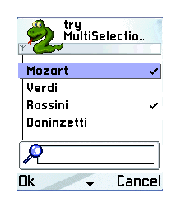
\includegraphics[width=\screenwidth]{markable-list}
\caption{Examples of a checkbox list (left) and a markable list (right)}
\label{fig:checkbox-and-markable-list}
\end{figure}

\subsection{Application Type}
\label{subsec:application}
A single implicit instance of this type always exists when \module{appuifw} 
module is present and can be referred to with the name \code{app}. New 
instances cannot be created by a Python program.

\begin{classdesc*}{Application}
Instances of \class{Application} type have the following attributes:

\begin{memberdesc}[Application]{body}
The UI control that is visible in the application's main window. Currently 
either \class{Text}, a \class{Listbox} object, \class{Canvas}, or 
\code{None}.
\end{memberdesc}

\begin{memberdesc}[Application]{exit_key_handler}
A callable object that is called when the user presses the Exit softkey. 
Setting \member{exit_key_handler} to \code{None} sets it back to the 
default value.
\end{memberdesc}

\begin{memberdesc}[Application]{menu}
This is a list of the following kinds of items:
\begin{itemize}
\item \code{(title, callback)} which creates a regular menu item
\item \code{(title, ((title, callback)\optional{...}))} which creates a submenu
\end{itemize}

\var{title} (Unicode) is the name of the item and \var{callback} the associated callable object. 
The maximum allowed number of items in a menu, or items in a submenu,
or submenus in a menu is 30.

Example:
\begin{verbatim}
appuifw.app.menu = [(u"Item 1", item1),
                    (u"Submenu 1", 
                        ((u"Subitem 1", subitem1),
                         (u"Subitem 2", subitem2)))]
\end{verbatim}
\end{memberdesc}

\begin{memberdesc}[Application]{screen}
The screen area used by an application. See \figurename~\ref{fig:alternate-uilayouts} for
example screens. The appearance of the application on the screen can
be affected by setting one of the following values: \code{'normal'},
\code{'large'}, and \code{'full'}.

Examples:
\begin{verbatim}
appuifw.app.screen='normal' # (a normal screen with title pane and softkeys)
appuifw.app.screen='large'  # (only softkeys visible)
appuifw.app.screen='full'   # (a full screen)
\end{verbatim}
\end{memberdesc}

\begin{memberdesc}[Application]{title}
The title the application that is visible in the application's title
pane. Must be Unicode.
\end{memberdesc}

\begin{memberdesc}[Application]{focus}
A callable object that is called with integer as parameter (0 = focus lost, 
1 = focus regained) when the application receives focus or it is switched to 
background. Focus is received e.g. when the application is switched from 
background to foreground or when the focus is regained from screensaver. 
Similarly when the screensaver is displayed, focus is lost.

Examples:
\begin{verbatim}
>>> import appuifw
>>> def cb(fg):
...   if(fg):
...     print "foreground"
...   else:
...     print "background"
...
>>> appuifw.app.focus=cb
>>> # switch to background, following text is printed from callback:
>>> background
>>> # switch to foreground, following text is printed from callback:
>>> foreground
\end{verbatim}

\begin{notice}
An improper callback can cause adverse effects. If you, for example,
define a callback which takes no parameters you will receive
never-ending \exception{TypeError} exceptions on the Nokia 6600.
\end{notice}

\end{memberdesc}

Instances of \class{Application} type have the following methods:

\begin{methoddesc}[Application]{activate_tab}{index}
Activates the tab \var{index} counting from zero.
\end{methoddesc}

\begin{methoddesc}[Application]{full_name}{}
Returns the full name, in Unicode, of the native application in whose 
context the current Python interpreter session runs.
\end{methoddesc}

\begin{methoddesc}[Application]{set_exit}{}
Requests a graceful exit from the application as soon as the current script 
execution returns.
\end{methoddesc}

\begin{methoddesc}[Application]{set_tabs}{tab_texts\optional{,callback=None}}
Sets tabs with given names on them in the navigation bar; 
\var{tab_texts} is a list of Unicode strings. When the users 
navigate between tabs, \var{callback} gets called with the index 
of the active tab as an argument. Tabs can be disabled by giving an empty or 
one-item \var{tab_texts} list.
\end{methoddesc}

\end{classdesc*}

\subsection{Form Type}
\label{subsec:form}
\class{Form} implements a dynamically configurable, editable multi-field 
dialog. \class{Form} caters for advanced dialog use cases with requirements 
such as free selectability of the combination of fields, possibility of 
validating the user input, and automatically producing the contents of some 
dialog fields before allowing the closing of the dialog. 

\begin{classdesc}{Form}{fields\optional{, flags=0}}
Creates a \class{Form} instance.
\var{fields} is a list of \emph{field descriptors}: \code{(label, type\optional{, value})} where

\var{label} is a Unicode string

\var{type} is one of the following strings: 
\code{'text'}, \code{'number'}, \code{'date'}, \code{'time'}, \code{'combo'}
or \code{'float'}

\var{value}, depending on \var{type}: Unicode string, numeric, float (seconds 
since Unix epoch rounded down to the nearest local midnight), float (seconds 
since local midnight), \code{([choice_label ...], index)} of float. For 
\code{'float'} \var{type} the initial value setting might not be shown in the 
UI.
\end{classdesc}

\class{Form} can also be configured and populated after construction. The 
configuration flags are visible as an attribute. \class{Form} implements 
the list protocol that can be used for setting the form fields, as well as 
obtaining their values after the dialog has been executed.

Instances of \class{Form} type have the following attributes:

\begin{memberdesc}[Form]{flags}
This attribute holds the values of the various configuration flags. 
Currently supported flags are:

\begin{datadesc}{FFormEditModeOnly}
When this flag is set, the form remains in edit mode while \method{execute} 
runs.
\end{datadesc}

\begin{datadesc}{FFormViewModeOnly}
When this flag is set, the form cannot be edited at all.
\end{datadesc}

\begin{datadesc}{FFormAutoLabelEdit}
This flag enables support for allowing the end-users to edit the labels of 
the form fields.
\end{datadesc}

\begin{datadesc}{FFormAutoFormEdit}
This flag enables automatic support for allowing the end-users to add and 
delete the form fields. Note that this is an experimental feature and is not 
guaranteed to work with all SDK versions.
\end{datadesc}

\begin{datadesc}{FFormDoubleSpaced}
When this flag is set, double-spaced layout is applied when the form is 
executed: one field takes two lines, as the label and the value field are on 
different lines.
\end{datadesc}
\end{memberdesc}

\begin{memberdesc}[Form]{menu}
A list of \code{(title, callback)} pairs, where 
each pair describes an item in the form's menu bar that is active while the 
dialog is being executed. \var{title} (Unicode) is the name of 
the item and \var{callback} the associated callable object.
\end{memberdesc}

\begin{memberdesc}[Form]{save_hook}
This attribute can be set to a callable object that receives one argument 
and returns a Boolean value. It gets called every time the users want to 
save the contents of an executing \class{Form} dialog. A candidate list for 
new form content - a list representing the currently visible state of the 
UI - is given as an argument. The list can be modified by 
\member{save_hook}. If \member{save_hook} returns \code{True}, the 
candidate list is set as the new contents of the form. Otherwise, the form 
UI is reset to reflect the field list contained in \class{Form} object.
\end{memberdesc}

Instances of \class{Form} type have the following methods:

\begin{methoddesc}[Form]{execute}{}
Executes the dialog by making it visible on the UI.
\end{methoddesc}

\begin{methoddesc}[Form]{insert}{index, field_descriptor}
Inserts the field descriptor into the \class{Form} before the given \var{index}.
\end{methoddesc}

\begin{methoddesc}[Form]{pop}{}
Removes the last field descriptor from the \class{Form} and returns it.
\end{methoddesc}

\begin{methoddesc}[Form]{length}{}the number of field descriptors in the form.
\end{methoddesc}

The subscript notation \code{f[i]} can be used to access or modify the
i-th element of the form \code{f}. Same limitations as discussed above
in the context of the flag \constant{FFormAutoFormEdit} apply to
modifying a form while it is executing. The ability to change the
schema of a form while it is executing is an experimental feature.

\subsection{Text Type}
\label{subsec:mylabel5}
\class{Text} is a text editor UI control. For examples on the options 
available with \class{Text}, see Figure \ref{fig:text-styles}.

\begin{figure}[htbp]
\centering
\includegraphics[width=\screenwidth]{text-styles-1}
\includegraphics[width=\screenwidth]{text-styles-2}
\caption{Examples of the options available for Text type}
\label{fig:text-styles}
\end{figure}

Instances of \class{Text} type have the following attributes:

\begin{memberdesc}[Text]{color}
The color of the text. \code{color} supports the same color representation 
models as the \module{graphics} module. For the supported color 
representation models, see Section \ref{sec:graphics}.
\end{memberdesc}

\begin{memberdesc}[Text]{focus}
A Boolean attribute that indicates the focus state of the control. Editor 
control also takes the ownership of the navigation bar, and this feature is 
needed to enable the usage of this control in applications that use the 
navigation bar - for example, navigation tabs.
\end{memberdesc}

\begin{memberdesc}[Text]{font} 
The font of the text. There are two possible ways to set this attribute:

\begin{itemize}

\item Using a supported Unicode font, for example \code{u"Latin12"}. Trying to set a font which is not supported by the device has no effect. A list of supported fonts can be retrieved by using \function{appuifw.available_fonts}.

Example, setting font:
\begin{verbatim}
t = appuifw.Text()
t.font = u"albi17b" # sets font to Albi 17 bold
t.font = u"LatinPlain12" # sets font to Latin Plain 12
\end{verbatim}
\item Using one of the default device fonts that are associated with the following labels (plain strings):
\code{'annotation', 'title', 'legend', 'symbol', 'dense', 'normal'}
Example, setting font: 
\begin{verbatim}
t.font = "title" # sets font to the one used in titles
\end{verbatim}

Example, checking the currently set font: 
\begin{verbatim}
unicodeFont = t.font
\end{verbatim}
\end{itemize}

The attribute value retrieved is always a Unicode string. If the font has 
been set with a label, for example, \code{'title'}, the attribute will 
retrieve the font associated with that label. 
\end{memberdesc}

\begin{memberdesc}[Text]{highlight_color}
The highlight color of the text. \code{highlight_color} supports the 
same color representation models as the \module{graphics} module. For the 
supported color representation models, see Section \ref{sec:graphics}.
\end{memberdesc}

\begin{memberdesc}[Text]{style}
The style of the text. The flags for this attribute are defined in the 
\module{appuifw} module. These flags can be combined by using the binary 
operator \code{|}. The flags can be divided into two types: text style 
and text highlight. Text style flags can be freely combined with each other. 
However, one or more text style flags can be combined with only one text 
highlight flag. The flags are:

Text style:

\begin{datadesc}{STYLE_BOLD} 
Enables bold text.
\end{datadesc}

\begin{datadesc}{STYLE_UNDERLINE}
Enables underlined text.
\end{datadesc}

\begin{datadesc}{STYLE_ITALIC} 
Enables italic text.
\end{datadesc}

\begin{datadesc}{STYLE_STRIKETHROUGH } 
Enables strikethrough.
\end{datadesc}

Text highlight:

\begin{datadesc}{HIGHLIGHT_STANDARD}
Enables standard highlight.
\end{datadesc}

\begin{datadesc}{HIGHLIGHT_ROUNDED}
Enables rounded highlight.
\end{datadesc}

\begin{datadesc}{HIGHLIGHT_SHADOW}
Enables shadow highlight.
\end{datadesc}

Only one highlight is allowed to be used at once. Therefore, it is possible 
to combine only one highlight with one or more text styles.

Examples:
\begin{verbatim}
t = appuifw.Text()

# These and other similar values and combinations are valid:
t.style = appuifw.STYLE_BOLD
t.style = appuifw.STYLE_UNDERLINE
t.style = appuifw.STYLE_ITALIC
t.style = appuifw.STYLE_STRIKETHROUGH
t.style = (appuifw.STYLE_BOLD|
	   appuifw.STYLE_ITALIC|
	   appuifw.STYLE_UNDERLINE)

# These values are valid:
t.style = appuifw.HIGHLIGHT_STANDARD
t.style = appuifw.HIGHLIGHT_ROUNDED
t.style = appuifw.HIGHLIGHT_SHADOW

# This combination is NOT valid:
# Invalid code, do not try!
t.style = (appuifw.HIGHLIGHT_SHADOW|appuifw.HIGHLIGHT_ROUNDED)
\end{verbatim}
\end{memberdesc}

Instances of \class{Text} type have the following methods:

\begin{methoddesc}[Text]{add}{text}
Inserts the Unicode string \var{text} to the current cursor position.
\end{methoddesc}

\begin{methoddesc}[Text]{bind}{event_code, callback}
Binds the callable Python object \var{callback} to event
\var{event_code}. The key codes are defined in 
the \module{key_codes} library module. The call 
\code{bind(event_code, None)} clears an 
existing binding. In the current implementation the event is always
passed also to the underlying native UI control.
\end{methoddesc}

\begin{methoddesc}[Text]{clear}{}
Clears the editor.
\end{methoddesc}

\begin{methoddesc}[Text]{delete}{\optional{pos=0, length=len()}}
Deletes \var{length} characters of the text held by the editor control, 
starting from the position \var{pos}.
\end{methoddesc}

\begin{methoddesc}[Text]{get_pos}{}
Returns the current cursor position.
\end{methoddesc}

\begin{methoddesc}[Text]{len}{}
Returns the length of the text string held by the editor control.
\end{methoddesc}

\begin{methoddesc}[Text]{get}{\optional{pos=0, length=len()}}
Retrieves \code{length} characters of the text held by the editor control, 
starting from the position \var{pos}.
\end{methoddesc}

\begin{methoddesc}[Text]{set}{text}
Sets the text content of the editor control to Unicode string 
\var{text}.
\end{methoddesc}

\begin{methoddesc}[Text]{set_pos}{cursor_pos}
Sets the cursor to \var{cursor_pos}.
\end{methoddesc}

\subsection{Listbox Type}
\label{subsec:listbox}

\begin{figure}[htbp]
\centering
\includegraphics[width=\screenwidth]{listbox-with-icons}
\caption{Listbox with icons}
\label{fig:listbox-with-icons}
\end{figure}

An instance of this UI control type is visible as a listbox, also known as a 
list in Symbian, that can be configured to be a single-line item or a 
double-item listbox. Figure \ref{fig:listbox-with-icons} shows a single-line 
item Listbox with icons. For more information on the MBM and MIF formats, 
see Section \ref{subsec:icon}.

\begin{classdesc}{Listbox}{list, callback}
Creates a \class{Listbox} instance. A callable object 
\var{callback} gets called when a listbox selection has been 
made. \code{list} defines the content of the listbox and can be one of the 
following:

\begin{itemize}
\item A normal (single-line item) listbox: a list of Unicode strings, for example \code{[unicode_string item1, unicode_string item2]}
\item A double-item listbox: a two-element tuple of Unicode strings , for example \code{[(unicode_string item1, unicode_string item1description), (unicode_string item2, unicode_string item2description)]}
\item A normal (single-line item) listbox with graphics: a two-element tuple consisting of a Unicode string and an \class{Icon} object, for example \code{[(unicode_string item1, icon1), (unicode_string item2, icon2)]}.
\item A double-item listbox with graphics: a three-element tuple consisting of two Unicode strings and one \class{Icon} object, for example \code{[(unicode_string item1, unicode_string item1description, icon1), (unicode_string item2, unicode_string item2description, icon2)]}
\end{itemize}

Example: To produce a normal (single-line item) listbox with graphics:
\begin{verbatim}
icon1 = appuifw.Icon(u"z:\\system\\data\\avkon.mbm", 28, 29)
icon2 = appuifw.Icon(u"z:\\system\\data\\avkon.mbm", 40, 41)
entries = [(u"Signal", icon1),
           (u"Battery", icon2)]
lb = appuifw.Listbox(entries, lbox_observe)
\end{verbatim}
\end{classdesc}

Instances of \class{Listbox} type have the following methods:

\begin{methoddesc}[Listbox]{bind}{event_code, callback}
Binds the callable Python object \var{callback} to event 
\var{event_code}. The key codes are defined in 
the \module{key_codes} library module. The call
\code{bind(event_code, None)} clears an 
existing binding. In the current implementation the event is always passed 
also to the underlying native UI control.
\end{methoddesc}

\begin{methoddesc}[Listbox]{current}{}
Returns the currently selected item's index in the \class{Listbox}.
\end{methoddesc}

\begin{methoddesc}[Listbox]{set_list}{list\optional{, current}}
Sets the \class{Listbox} content to a list of Unicode strings or a
list of tuples of Unicode strings. The accepted structures of \var{list} are the
same as in the \class{Listbox} constructor. The optional argument \var{current} is the index of the focused list item.
\end{methoddesc}

\subsection{Icon Type}
\label{subsec:icon}
An instance of \class{Icon} type encapsulates an icon to be used together 
with a \class{Listbox} instance. Note that currently \class{Icon} can only 
be used with \class{Listbox} (see Section \ref{subsec:listbox}).

MBM is the native Symbian OS format used for pictures. It is a
compressed file format where the files can contain several bitmaps and
can be referred to by a number. An \code{.mbg} file is the header file
usually associated with an \code{.mbm} file, which includes symbolic
definitions for each bitmap in the file. For example, an
\file{avkon.mbm} file has an associated index file called
\file{avkon.mbg}, which is included in S60 SDKs. For more information
on the MBM format and the bitmap converter tool, see \cite{S60Doc} and
search the topics with the key term "How to provide Icons"; this topic
also points you to the Bitmap Converter tool that can be used for
converting bitmaps into the MBM format.

S60 2$^{nd}$ Edition FP3 introduces a new format for icons called 
Multi-Image File (MIF). This format is very similar to the MBM format and 
also contains several compressed files. The files to be compressed should be 
in Scalable Vector Graphics Tiny (SVG-T) format. For more information on the 
SVG format, see Scalable Vector Graphics (SVG) 1.1 Specification 
[10].

\begin{classdesc}{Icon}{filename, bitmap, bitmapMask}
Creates an icon. \var{filename} is a Unicode file name and must 
include the whole path. Note that MBM and MIF (MIF only in S60 2nd 
Edition FP3) are the only file formats supported. \var{bitmap} 
and \var{bitmapMask} are integers that represent the index of 
the icon and icon mask inside that file respectively.
\end{classdesc}

Example: The following builds an icon with the standard signal symbol:
\begin{verbatim}
icon = appuifw.Icon(u"z:\\system\\data\\avkon.mbm", 28, 29)
\end{verbatim}

\subsection{Content_handler Type}
\label{subsec:content}

An instance of \class{Content_handler} handles data content by its MIME 
type.

\begin{classdesc}{Content_handler}{\optional{callback}}
Creates a \class{Content_handler} instance. A Content_handler handles
data content by its MIME type. The optional
\var{callback} is called when the embedded handler application 
started with the \method{open} method finishes. 
\end{classdesc}

Instances of \class{Content_handler} type have the following methods:

\begin{methoddesc}[Content_handler]{open}{filename}
Opens the file \var{filename} (Unicode) in its handler 
application if one has been registered for the particular MIME type. The 
handler application is embedded in the caller's thread. The call to this 
function returns immediately. When the handler application finishes, the 
\var{callback} that was given to the \class{Content_handler} 
constructor is called.
\end{methoddesc}

\begin{methoddesc}[Content_handler]{open_standalone}{filename}
Opens the file \var{filename} (Unicode) in its handler 
application if one has been registered for the particular MIME type. The 
handler application is started in its own process. The call to this function 
returns immediately. Note that \var{callback} is not called for 
applications started with this method.
\end{methoddesc}

\subsection{Canvas Type}
\label{subsec:canvas}
\class{Canvas} is a UI control that provides a drawable area on the screen 
and support for handling raw key events. \class{Canvas} supports the 
standard drawing methods that are documented in Section \ref{sec:graphics}.

\begin{classdesc}{Canvas}{\optional{redraw_callback=None, event_callback=None}}
Constructs a \class{Canvas}. The optional parameters are callbacks
that are called when specific events occur. 

\note{Watch out for cyclic
references here. For example, if the callbacks are methods of an
object that holds a reference to the \class{Canvas}, a reference cycle
is formed that must be broken at cleanup time or the
\class{Canvas} will not be freed.}

\var{redraw_callback} is called whenever a part of the \class{Canvas} 
has been obscured by something, is then revealed, and needs to be
redrawn. This can typically happen, for example, when the user
switches away from the Python application and back again, or after
displaying a pop-up menu. The callback takes as its argument a
four-element tuple that contains the top-left and the bottom-right
corner of the area that needs to be redrawn. In many cases redrawing
the whole
\class{Canvas} is a reasonable option. 

\var{event_callback} is called whenever a raw key event is received.
There are three kinds of key events: \code{EEventKeyDown},
\code{EEventKey}, and \code{EEventKeyUp}. When a user presses a key 
down, events \code{EEventKeyDown} and \code{EEventKey} are generated. 
When the key is released, an \code{EEventKeyUp} event is generated.

The argument to the \var{event_callback} is a dictionary that contains 
the following data for key events:

\begin{itemize}
\item \code{'type'}: one of \code{EEventKeyDown}, \code{EEventKey}, or \code{EEventKeyUp}
\item \code{'keycode'}: the keycode of the key
\item \code{'scancode'}: the scancode of the key
\item \code{'modifiers'}: the modifiers that apply to this key event
\end{itemize}

Each key on the keyboard has one or more scancodes and zero or more keycodes 
associated with it. A scancode represents the physical key itself and a 
keycode is the result of state-related operating system defined processing 
done on the key. For keys that correspond to a symbol in the current 
character set of the phone, the keycode is equal to the code of the 
corresponding symbol in that character set. For example, if you are using 
the Nokia Wireless Keyboard (SU-8W), pressing the key A will always produce 
the scancode 65 (ASCII code for an upper case A), but the keycode 
could be either 65 or 91 (ASCII code for a lower case A) depending on 
whether or not the Shift key is pressed or Caps Lock is active. 

The \module{key_codes} module contains definitions for the keycodes and 
scancodes. See \figurename~\ref{fig:keyboard} for the codes of the most 
common keys on the phone keypad. 

Some keys are handled in a special way:

\begin{itemize}
\item A short press of the Edit key causes it to stay down, meaning that no \code{EEventKeyUp} event is sent. The event is only sent after a long press.
\item Detecting presses of the Voice tags key or the Power key is not supported.
\item If the right softkey is pressed, the \code{appuifw.app.exit_key_handler} callback is always executed.
\end{itemize}

There is no way to prevent the standard action of the Hang-up key, the Menu 
key, the Power key or the Voice tags key from taking place.

\begin{figure}
\centering
\includegraphics[width=5in]{6630keyboard}
%\includegraphics[width=3.60in,height=2.58in]{6630keyboard}
%\centerline{\includegraphics[width=3.60in,height=2.58in]{API_Reference_for_Python11.eps}} \par & 
\begin{tableiii}{lll}{textrm}{Key}{Keycode}{Scancode}
\lineiii{1.}{EKeyLeftSoftkey}{EScancodeLeftSoftkey}
\lineiii{2.}{EKeyYes}{EScancodeYes}
\lineiii{3.}{EKeyMenu}{EScancodeMenu}
\lineiii{4.}{EKey0...9}{EScancode0...9}
\lineiii{5.}{EKeyStar}{EScancodeStar}
\lineiii{6.}{EKeyLeftArrow}{EScancodeLeftArrow}
\lineiii{7.}{EKeyUpArrow}{EScancodeUpArrow}
\lineiii{8.}{EKeySelect}{EScancodeSelect}
\lineiii{9.}{EKeyRightArrow}{EScancodeRightArrow}
\lineiii{10.}{EKeyDownArrow}{EScancodeDownArrow}
\lineiii{11.}{EKeyRightSoftkey}{EScancodeRightSoftkey}
\lineiii{12.}{EKeyNo}{EScancodeNo}
\lineiii{13.}{EKeyBackspace}{EScancodeBackspace}
\lineiii{14.}{EKeyEdit}{EScancodeEdit}
\lineiii{15.}{EKeyHash}{EScancodeHash}
\end{tableiii}
\caption{Keycodes and scancodes for phone keys usable from Python applications}
\label{fig:keyboard}
\end{figure}

\end{classdesc}

Instances of \class{Canvas} type have the following attribute:

\begin{memberdesc}[Canvas]{size}
A two-element tuple that contains the current width and height of the 
\class{Canvas} as integers.
\end{memberdesc}

Instances of \class{Canvas} type have the same standard drawing methods 
that are documented in Section \ref{sec:graphics}.

\input{libgraphics}
% Copyright (c) 2005 Nokia Corporation
%
% Licensed under the Apache License, Version 2.0 (the "License");
% you may not use this file except in compliance with the License.
% You may obtain a copy of the License at
%
%     http://www.apache.org/licenses/LICENSE-2.0
%
% Unless required by applicable law or agreed to in writing, software
% distributed under the License is distributed on an "AS IS" BASIS,
% WITHOUT WARRANTIES OR CONDITIONS OF ANY KIND, either express or implied.
% See the License for the specific language governing permissions and
% limitations under the License.

\section{\module{camera} ---
    Interface for taking photographs}

\declaremodule{extension}{camera}
\label{sec:camera}

\begin{notice}[note]
Not available for S60 1st Edition.
\end{notice}

The \module{camera} module enables taking photographs. 

The \module{camera} module has the following functions\footnote{ 
Descriptions for some of the values are based on information found in S60 SDK documentation \cite{S60Doc}}:

\begin{funcdesc}{cameras_available}{}
Returns the number of cameras available in the device.
\end{funcdesc}

\begin{funcdesc}{image_modes}{}
Returns the image modes supported in the device as a list of strings, for 
example: \code{['RGB12', 'RGB', 'RGB16'].}
\end{funcdesc}

\begin{funcdesc}{image_sizes}{}
Returns the image sizes (resolution) supported in the device as a list of 
\code{(x, y)} tuples, for example: \code{[(640, 480), (160, 120)]}.
\end{funcdesc}

\begin{funcdesc}{flash_modes}{}
Returns the flash modes available in the device as a list of strings. 
\end{funcdesc}

\begin{funcdesc}{max_zoom}{}
Returns the maximum digital zoom value supported in the device as an 
integer. 
\end{funcdesc}

\begin{funcdesc}{exposure_modes}{}
Returns the exposure settings supported in the device as a list of strings. 
\end{funcdesc}

\begin{funcdesc}{white_balance_modes}{}
Returns the white balance modes available in the device as a list of 
strings. 
\end{funcdesc}

\begin{funcdesc}{take_photo}{\optional{mode, size, flash, zoom, exposure, white_balance, position}}
Takes a photograph and returns the image in \code{Image} format (for more 
information on \code{Image} format, see Chapter \ref{sec:graphics} 
\refmodule{graphics} Module). If some other application is using the camera, 
this operation fails, for example with \code{SymbianError: KErrInUse}. The 
settings listed below describe all settings that are supported by the 
\code{camera} module. You can retrieve the mode settings available for your 
device by using the appropriate functions listed at the beginning of this 
chapter.

\begin{itemize}
\item \var{mode} is the display mode of the image. The default value is \code{'RGB16'}. The following display modes are supported:
	\begin{itemize}
	\item \code{'RGB12'}: 4096 colors (12 bits per pixel)
	\item \code{'RGB16'}: 65536 colors (16 bits per pixel). Default value, always supported
	\item \code{'RGB'}: 16.7 million colors (24 bits per pixel)
	\end{itemize}
\item \var{size} is the resolution of the image. The default value is \code{(640, 480)}. The following sizes are supported, for example, in Nokia 6630: \code{(1280, 960)}, \code{(640, 480)} and \code{(160, 120)}.
\item \var{flash} is the flash mode setting. The default value is \code{'none'}. The following flash mode settings are supported:
	\begin{itemize}
	\item \code{'none' \newline
}No flash. Default value, always supported
	\item \code{'auto' \newline
}Flash will automatically fire when required
	\item \code{'forced' \newline
}Flash will always fire
	\item \code{'fill_in' \newline
}Reduced flash for general lighting
	\item \code{'red_eye_reduce' \newline
}Red-eye reduction mode
	\end{itemize}
\item \var{zoom} is the digital zoom factor. It is assumed to be on a linear scale from 0 to the maximum zoom value allowed in the device. The default value is \code{0}, meaning that zoom is not used. 
\item \var{exposure} is the exposure adjustment of the device. Exposure is a combination of lens aperture and shutter speed used in taking a photograph. The default value is \code{'auto'.} The following exposure modes are supported:
	\begin{itemize}
	\item \code{'auto'} \newline
Sets exposure automatically. Default value, always supported
	\item \code{'night'} \newline
Night-time setting for long exposures
	\item \code{'backlight' } \newline
Backlight setting for bright backgrounds
	\item \code{'center'} \newline
Centered mode for ignoring surroundings
	\end{itemize}
\item \var{white_balance} can be used to adjust white balance to match the main source of light. The term white balance refers to the color temperature of the current light. A digital camera requires a reference point to represent white. It will then calculate all the other colors based on this white point. The default value for \var{white_balance} is \code{'auto'} and the following white balance modes are supported:
	\begin{itemize}
	\item \code{'auto'} \newline
Sets white balance automatically. Default value, always supported
	\item \code{'daylight'} \newline
Sets white balance to normal daylight
	\item \code{'cloudy}' \newline
Sets white balance to overcast daylight
	\item \code{'tungsten'} \newline
Sets white balance to tungsten filament lighting
	\item \code{'fluorescent}' \newline
Sets white balance to fluorescent tube lighting
	\item \code{'flash'} \newline
Sets white balance to flash lighting
	\end{itemize}
\item \var{position} is the camera used if the device, such as Nokia 6680, has several cameras. In Nokia 6680, the camera pointing to the user of the device is located in position \code{1}, whereas the one pointing away from the user is located in position \code{0}. The default \var{position} is \code{0}.
\end{itemize}
\end{funcdesc}


\chapter{Audio and Communication Services \label{s60ac}}

\input{libaudio}
% Copyright (c) 2005 Nokia Corporation
%
% Licensed under the Apache License, Version 2.0 (the "License");
% you may not use this file except in compliance with the License.
% You may obtain a copy of the License at
%
%     http://www.apache.org/licenses/LICENSE-2.0
%
% Unless required by applicable law or agreed to in writing, software
% distributed under the License is distributed on an "AS IS" BASIS,
% WITHOUT WARRANTIES OR CONDITIONS OF ANY KIND, either express or implied.
% See the License for the specific language governing permissions and
% limitations under the License.

\section{\module{telephone} ---
	 Telephone services}
\label{sec:telephone}

\declaremodule{extension}{telephone}
\platform{S60}
\modulesynopsis{A telephone related services package.}

This module provides an API to a telephone. 

Since the users of the device can also hang-up the phone explicitly, they 
might affect the current status of the call. In addition, using this 
extension in an emulator has no effect since no calls can be connected.

The \module{telephone} module has the following functions:

\begin{funcdesc}{dial}{number}

Dials the number set in \var{number}. \var{number} 
is a string, for example \code{u'+358501234567'} where \code{'+'} is the 
international prefix, \code{'358'} is the country code, \code{'50'} is 
the mobile network code (or the area code), and \code{'1234567'} is the 
subscriber number. If there is an ongoing phone call prior to calling 
\method{dial} from Python, then the earlier call is put on hold and a new 
call is established. Calling \method{dial} multiple times when, for example, 
the first call has been answered and a line has been established results in 
subsequent calls not being connected.
\end{funcdesc}

\begin{funcdesc}{hang\_up}{}
Hangs up if a call initiated by \method{dial} is in process. If this call 
has already been finished, \exception{SymbianError: KErrNotReady} is raised.
\end{funcdesc}

\input{libmessaging}
\input{libinbox}
\input{liblocation}

\chapter{Data Management \label{s60data}}

\input{libcontacts}
\input{libcalendar}
\input{libe32db}
\input{libe32dbm}

\chapter{Standard Library Support and Extensions \label{s60lib}}

% Copyright (c) 2005 Nokia Corporation
%
% Licensed under the Apache License, Version 2.0 (the "License");
% you may not use this file except in compliance with the License.
% You may obtain a copy of the License at
%
%     http://www.apache.org/licenses/LICENSE-2.0
%
% Unless required by applicable law or agreed to in writing, software
% distributed under the License is distributed on an "AS IS" BASIS,
% WITHOUT WARRANTIES OR CONDITIONS OF ANY KIND, either express or implied.
% See the License for the specific language governing permissions and
% limitations under the License.

\section{Support for Python Standard Library}
\label{sec:standard}

The standard library support in Python for S60 is summarized in Table 
\ref{standardsupport}. For API descriptions, see \cite{PyLibRef}.

\begin{center}
\begin{longtable}{|l|l|l|p{200pt}|}
\hline
{\bf Name}& 
{\bf Type}& 
{\bf Status}& 
{\bf Remarks} \\
\hline
\code{{\_}testcapi}& 
PYD& 
Y& 
 \\
\hline
\code{anydbm}& 
PY& 
X& 
DBM API is implemented by PY \code{e32dbm} that relies on PYD \code{e32db} (see Chapter \ref{sec:e32dbm}, e32dbm Module) \\
\hline
\code{atexit}& 
PY& 
X& 
 \\
\hline
\code{base64}& 
PY& 
X& 
 \\
\hline
\code{bdb}& 
PY& 
(X)& 
 \\
\hline
\code{binascii}& 
built-in& 
X& 
 \\
\hline
\code{cmd}& 
PY& 
(X)& 
 \\
\hline
\code{code}& 
PY& 
X& 
 \\
\hline
\code{codecs}& 
PY& 
X& 
 \\
\hline
\code{codeop}& 
PY& 
X& 
 \\
\hline
\code{copy}& 
PY& 
X& 
 \\
\hline
\code{copy{\_}reg}& 
PY& 
X& 
 \\
\hline
\code{cStringIO}& 
built-in& 
X& 
 \\
\hline
\code{dis}& 
PY& 
(X)& 
 \\
\hline
\code{errno}& 
built-in& 
X& 
 \\
\hline
\code{exceptions}& 
built-in& 
X& 
 \\
\hline
\code{{\_}{\_}future{\_}{\_}}& 
PY& 
X& 
 \\
\hline
\code{httplib}& 
PY& 
X& 
 \\
\hline
\code{imp}& 
built-in& 
X& 
 \\
\hline
\code{keyword}& 
PY& 
X& 
 \\
\hline
\code{linecache}& 
PY& 
X& 
 \\
\hline
\code{marshal}& 
built-in& 
X& 
 \\
\hline
\code{math}& 
built-in& 
X& 
 \\
\hline
\code{md5}\footnote{Derived from the RSA Data Security, Inc. MD5 Message-Digest Algorithm.}& 
built-in& 
X& 
 \\
\hline
\code{mimetools}& 
PY& 
X& 
 \\
\hline
\code{operator}& 
built-in& 
X& 
 \\
\hline
\code{os, os.path}& 
PY& 
X& 
Wraps built-in \code{e32posix}. Limitations discussed in Section \ref{subsec:limitations}, Limitations and Areas of Development. \\
\hline
\code{pdb}& 
PY& 
(X)& 
 \\
\hline
\code{quopri}& 
PY& 
X& 
 \\
\hline
Name& 
Type& 
Status& 
Remarks \\
\hline
\code{random}& 
PY& 
X& 
 \\
\hline
\code{re}& 
PY& 
X& 
Uses PY \code{sre} as its engine. \\
\hline
\code{repr}& 
PY& 
X& 
 \\
\hline
\code{rfc822}& 
PY& 
X& 
 \\
\hline
\code{select}& 
PY& 
X& 
A minimal implementation: \code{select} is supported only for input from sockets. \\
\hline
\code{socket}& 
PY& 
X& 
Requires PYD \code{e32socket}. Contains extensions as described in Section \ref{subsec:socket}, socket Module. Limitations discussed in Section \ref{subsec:limitations}, Limitations and Areas of Development.  \\
\hline
\code{sre}& 
PY& 
X& 
Wraps built-in \code{{\_}sre}. \\
\hline
\code{string}& 
PY& 
X& 
 \\
\hline
\code{StringIO}& 
PY& 
X& 
 \\
\hline
\code{struct}& 
built-in& 
X& 
 \\
\hline
\code{sys}& 
built-in& 
X& 
 \\
\hline
\code{thread}& 
built-in& 
X& 
Contains extensions as described in Section \ref{subsec:thread}, thread Module \\
\hline
\code{threading}& 
PY& 
(X)& 
 \\
\hline
\code{time}& 
built-in& 
X& 
 \\
\hline
\code{traceback}& 
PY& 
X& 
 \\
\hline
\code{types}& 
PY& 
X& 
 \\
\hline
\code{urllib}& 
PY& 
X& 
 \\
\hline
\code{urlparse}(urlsplit only)& 
PY& 
X& 
 \\
\hline
\code{uu}& 
PY& 
X& 
 \\
\hline
\code{warnings}& 
PY& 
X& 
 \\
\hline
\code{whichdb}& 
PY& 
X& 
 \\
\hline
\code{xreadlines}& 
built-in& 
X& 
 \\
\hline
\code{zipfile}& 
PY& 
X& 
 \\
\hline
\code{zlib}& 
PYD& 
X& 
 \\
\hline
\caption{Status of library module support.}
\label{standardsupport}
\end{longtable}
\end{center}

Table \ref{standardsupport} uses the following coding for module types:

\begin{itemize}
\item PY -- module is implemented in Python.
\item Built-in -- module is a built-in C/C++ module.
\item PYD -- module is a dynamically loadable C/C++ module.
\end{itemize}
For support status, the following codes are used:

\begin{enumerate}
\item[\textbullet] X -- included to the Series 60 Python distribution.
\item[\textbullet] (X) -- not included to the Series 60 Python distribution, but works both on phone and SDK.
\item[\textbullet] Y -- included only to the SDK distribution.
\end{enumerate}


\section{Extensions to Standard Library Modules}
\label{extensions}

The following standard modules have been extended.

\subsection{\module{thread} ---
  S60 extensions to standard thread module} 
\label{subsec:thread}

\declaremodule{extension}{thread}
\modulesynopsis{S60 extensions to standard thread module.}

The following function has been added to the standard \code{thread} 
module:

\begin{funcdesc}{ao_waittid}{thread_id}

Synchronizes with the end of the execution of the thread identified by the given 
\var{thread_id}. The implementation is based on a Symbian OS active object. 
For the blocking behavior, see Section \ref{subsec:Aolock}, Ao_lock Type.

\end{funcdesc}

\subsection{\module{socket} ---
  S60 extensions to standard socket module} 
\label{subsec:socket}

\declaremodule{extension}{socket}
\modulesynopsis{Extensions to standard socket module.}

Bluetooth (BT) support has been added to the standard \code{socket} 
module. The following related constants and functions are defined:

\begin{notice}[note]
In release 1.0 the functions \code{bt_advertise_service}, 
\code{bt_obex_receive}, and 
\code{bt_rfcomm_get_available_server_channel} incorrectly 
expected to be given the internal \code{e32socket.socket} object as the 
socket parameter instead of the proper \code{socket} object. Now the 
functions work correctly. The old calling convention is still supported but 
it is deprecated and may be removed in a future release.
\end{notice}

\begin{datadesc}{AF_BT}

Represents the Bluetooth address family.

\end{datadesc}

\begin{datadesc}{BTPROTO_RFCOMM}

This constant represents the Bluetooth protocol RFCOMM.

\end{datadesc}

\begin{datadesc}{RFCOMM}
\end{datadesc}
\begin{datadesc}{OBEX}

Bluetooth service classes supported by \code{bt_advertise_service}.

\end{datadesc}

\begin{datadesc}{AUTH}
\end{datadesc}
\begin{datadesc}{ENCRYPT}
\end{datadesc}
\begin{datadesc}{AUTHOR}

Bluetooth security mode flags.

\end{datadesc}

\begin{funcdesc}{bt_advertise_service}{name, socket, flag, class}

Sets a service advertising the service \var{name} (Unicode) on local channel 
that is bound to \var{socket}. If \var{flag} is \code{True}, the advertising is 
turned on, otherwise it is turned off. The service class to be advertised is 
either \code{RFCOMM} or \code{OBEX}.

\end{funcdesc}

\begin{funcdesc}{bt_discover}{\optional{address}}

Performs the Bluetooth device discovery (if the optional BT device address 
is not given) and the discovery of RFCOMM class services on the chosen 
device. Returns a pair: BT device address, dictionary of services, where 
Unicode service name is the key and the corresponding port is the value.

\end{funcdesc}

\begin{funcdesc}{bt_obex_discover}{\optional{address}}

Same as \code{discover}, but for discovery of OBEX class services on the 
chosen device.

\end{funcdesc}

\begin{funcdesc}{bt_obex_send_file}{address, channel, filename}

Sends file \var{filename} (Unicode) wrapped into an OBEX object 
to remote \var{address}, \var{channel}.

\end{funcdesc}

\begin{funcdesc}{bt_obex_receive}{socket, filename}

Receives a file as an OBEX object, unwraps and stores it into \var{filename} 
(Unicode). \var{socket} is a bound \code{OBEX} socket.

\end{funcdesc}

\begin{funcdesc}{bt_rfcomm_get_available_server_channel}{socket}

Returns an available RFCOMM server channel for \var{socket}.

\end{funcdesc}

\begin{funcdesc}{set_security}{socket, mode}

Sets the security level of the given bound \var{socket}. The 
\var{mode} is an integer flag that is formed using a binary 
\code{or} operation of one or more of: \code{AUTH} (authentication), 
\code{ENCRYPT}, \code{AUTHOR} (authorization). Example: 
\code{set_security(s, AUTH | AUTHOR)}.

\end{funcdesc}

\begin{notice}[note]
When listening to a Bluetooth socket on the phone, it is necessary to set 
the security level.
\end{notice}

\begin{notice}[note]
SSL is not supported in S60 1st Edition. SSL client certificates are 
not supported at all.
\end{notice}

For examples on the usage of these functions, see Programming with Python for 
S60 Platform \cite{PyS60Prog}.


\chapter{Extending and Embedding \label{s60ext}}

\input{capiextensions}
\input{extending}

\input{libabbreviations}
\input{libreferences}

\appendix

\chapter{Reporting Bugs}
\input{reportingbugs}


%  The ugly "%begin{latexonly}" pseudo-environments are really just to
%  keep LaTeX2HTML quiet during the \renewcommand{} macros; they're
%  not really valuable.


%begin{latexonly}
\renewcommand{\indexname}{Module Index}
%end{latexonly}
\input{modlib.ind}              % Module Index

%begin{latexonly}
\renewcommand{\indexname}{Index}
%end{latexonly}
% Portions Copyright (c) 2005 Nokia Corporation
\documentclass{manual}

% NOTE: this file controls which chapters/sections of the library
% manual are actually printed.  It is easy to customize your manual
% by commenting out sections that you're not interested in.

\title{PyS60 Library Reference}

\input{boilerplate}

\makeindex                      % tell \index to actually write the
                                % .idx file
\makemodindex                   % ... and the module index as well.

%begin{latexonly}
\ifx\pdftexversion\undefined
 \usepackage[dvips]{graphicx}
\else
 \usepackage[pdftex]{graphicx}
\fi
%end{latexonly}
\usepackage{graphicx}

\usepackage{longtable}

\graphicspath{{./}{figures/}}

\begin{document}

\maketitle

\ifhtml
\chapter*{Front Matter\label{front}}
\fi

\input{copyright}

\begin{abstract}

\noindent

The Python for S60 Platform (Python for S60) simplifies application development 
and provides a scripting solution for the Symbian C++ APIs. This document is for 
Python for S60 version \productversion that is based on Python 2.2.2.

\end{abstract}

\tableofcontents

                                % Chapter title:

\input{libintro}                % Introduction

\input{libsummary}              % API summary

\input{libselected}             % Selected issues

\chapter{Operating System Services and Information \label{s60os}}

\input{libe32}
\input{libsysinfo}

\chapter{User Interface and Graphics \label{s60graph}}

\input{libappuifw}
\input{libgraphics}
\input{libcamera}

\chapter{Audio and Communication Services \label{s60ac}}

\input{libaudio}
\input{libtelephone}
\input{libmessaging}
\input{libinbox}
\input{liblocation}

\chapter{Data Management \label{s60data}}

\input{libcontacts}
\input{libcalendar}
\input{libe32db}
\input{libe32dbm}

\chapter{Standard Library Support and Extensions \label{s60lib}}

\input{standardlibrary}
\input{libextensions}

\chapter{Extending and Embedding \label{s60ext}}

\input{capiextensions}
\input{extending}

\input{libabbreviations}
\input{libreferences}

\appendix

\chapter{Reporting Bugs}
\input{reportingbugs}


%  The ugly "%begin{latexonly}" pseudo-environments are really just to
%  keep LaTeX2HTML quiet during the \renewcommand{} macros; they're
%  not really valuable.


%begin{latexonly}
\renewcommand{\indexname}{Module Index}
%end{latexonly}
\input{modlib.ind}              % Module Index

%begin{latexonly}
\renewcommand{\indexname}{Index}
%end{latexonly}
\input{lib.ind}                 % Index

\end{document}
                 % Index

\end{document}
                 % Index

\end{document}
                 % Index

\end{document}
